\chapter{Alvorada}
\label{ch:proposta}

Este capítulo destina-se a explanar a proposta para o problema apresentado. De antemão são apresentadas as escolhas de arquitetura realizadas, referentes aos tópicos levantados no Capítulo \ref{ch:fundamentos}. Para simplificar o entendimento do protocolo uma série de informações iniciais a seu respeito são apresentadas. Na Seção \ref{sec:proposta:atores} são apresentados todos os atores que compõem a rede e como esses podem se comunicar através da cadeia. A Seção \ref{sec:proposta:definicoes} apresenta um panorama geral das características técnicas e estruturais do protocolo, bem como as peculiaridades da \textit{Blockchain} proposta. Aspectos sobre o cenário de execução do protocolo são mostrados na Seção \ref{sec:cenario_execucao} e um modelo da execução em si é apresentado nas Seções \ref{sec:proposta:fase_contratual} e \ref{sec:proposta:fase_auditoria}, definindo os processos envolvidos na elaboração de contratos e nas suas auditorias, respectivamente. Por fim na Seção \ref{sec:trabalhos_relacionados}, são apresentados os trabalhos que possuem relação com o foco de resolução da presente proposta.

% A Seção \ref{sec:proposta:exemplo} apresenta um exemplo prático do funcionamento e por fim, após a definição do protocolo, são apresentadas na Seção \ref{sec:proposta:ameacas} ameaças que podem afetar seu funcionamento correto.

% TODO: ajustar o texto após a reorganização. A Seção 3.7 será transformada em novo capítulo.

% as justificativas a respeito de cada escolha são explanadas na Seção \ref{}. 

%
\section{Atores Participantes}
\label{sec:proposta:atores}

Mediante à execução do protocolo, diferentes atores participantes interagem com a cadeia. Estes possuem diferentes poderes e possibilidades de escrita:
\begin{itemize}
    \item Os clientes formam o primeiro grupo de atores, que entram na rede em busca da escolha de um provedor que atenda aos seus padrões de preço, qualidade de serviço e reputação para realizar a alocação de microsserviços. Seus poderes envolvem o pedido devidamente organizado de uma alocação para a rede, a confirmação de propostas de provedores, prolongação de requisições, convocações de votação para possíveis quebras de contrato e o voto em convocações de outros usuários contra o seu provedor.
    \item O segundo grupo de participantes são os prestadores de serviço, que adentram a rede em busca de novos clientes. Seus poderes envolvem responder a pedidos de alocação com propostas para um ou mais microsserviços distintos e votar em convocações para outros usuários do mesmo grupo. O termo prestador de serviço foi empregado de modo a generalizar o entendimento desse usuário, que pode ser a manifestação de um provedor ou de um corretor.
\end{itemize}

A partir do presente momento, qualquer participante da rede é referido apenas como usuário, independentemente do grupo de atores do qual faz parte. Cada usuário, representado por um endereço que trata-se de sua chave pública atual, pode pertencer apenas a um dos grupos de atores, sendo essa informação definida quando o indivíduo entra na rede e naturalmente não podendo ser modificada posteriormente. Assim, ficam claras as funções diretamente ligadas a cada um dos tipos de usuário: clientes criam usuários do tipo cliente para que possam comprar serviços e provedores criam usuários do tipo prestador de serviço para vendê-los, de forma que esses são seus únicos poderes individuais mutuamente excludentes. Corretores entretanto, não se encaixam de forma completa em nenhum dos dois grupos e para exercer corretamente suas funções mercadológicas deveriam compartilhar funções de ambos. Para tal, corretores devem possuir dois usuários distintos um pertencente ao grupo de clientes para que possa adquirir serviços e outro pertence aos prestadores de serviço, para revendê-los. 

%
Essa abordagem embora relativamente simples apresenta vantagens significativas quando comparada a outras possíveis soluções como por exemplo o uso de um grupo de usuários específicos para corretores. Primeiramente, o protocolo torna-se mais segregado no que diz respeito às possibilidades de ação dos usuários onde um grupo apenas compra e outro apenas vende, consequentemente o processo de implementação torna-se mais simples e é prevenida a existência de transações extras ou mecanismos especializados para o tratamento de informações ou negociações com um terceiro grupo de usuários. A segunda grande vantagem é a culpabilidade que a abordagem proporciona, pois se um corretor for acusado da violação de um contrato e perder reputação, mas o verdadeiro culpado é o provedor dono da infraestrutura contratada, é possível que o corretor em questão utilize sua conta de usuário - pelo qual a contratação foi feita - para convocar uma votação denunciando o provedor e retomando sua reputação. Contudo, caso o verdadeiro culpado seja realmente o corretor, não seria possível que ele transferisse sua culpa para o provedor porque nem ele e nem os outros participantes da rede possuiriam dados de monitoração condizentes com a acusação, impossibilitando a vitória na votação. 

%
Outro fator interessante dessa forma de organização da rede é a possibilidade da existência de encadeamento do serviços, no qual um provedor inicial pode vender infraestruturas para um corretor, que pode novamente repassá-las para outro corretor, sendo que este também pode possuir outra parte de sua infraestrutura adquirida de um provedor e assim por diante. Consequentemente, um grande número de cenários mercadológicos heterogêneos podem surgir, bem como árvores de serviço e repasse podem ser estabelecidas para a posterior venda a clientes finais.

\section{Definições Iniciais da Rede}
\label{sec:proposta:definicoes}

Como explanado na Seção~\ref{subsec:blobkchain:transacaoes}, o conceito de \textit{Blockchain} em si é flexível e permite diferentes formas de implementação. Assim o protocolo proposto baseia-se no \textit{Bitcoin}, principalmente por fazer uso do conceito de transações não gastas, que na implementação original servem como registro das moedas pertencentes a um usuário, mas nesse contexto são interessantes por permitirem uma noção de estados completos e incompletos. Portanto, transações ainda não respondidas - gastas como entrada - por um determinado usuário podem representar processos que ainda não foram concluídos como aberturas para votações ou propostas para um serviço, enquanto a resposta a uma transação anterior por uma atual pode indicar o fim de certo processo anteriormente aberto.

%
O termo transação é empregado recorrentemente no decorrer desse trabalho para se referir as mensagens trocadas através da cadeia. Entretanto, a rede proposta não tem seu fim em transações monetárias, assim não trata-se de uma criptomoeda em essência, porém utilizam-se certas características normalmente adotadas nelas em conjunto com propriedades destoantes que melhor refletem as necessidades do problema abordado.

%
A maioria das informações que transitam entre os usuários e que consequentemente são escritas na cadeia se referem puramente a dados de definição e concretização de contratos, desenvolvidas para otimizar e facilitar o processo de contratação de infraestruturas, bem como para possível avaliação posterior.
%
Apenas uma pequena parcela do total de transações conterá movimentação de valores propriamente ditos e estes não servirão como moeda de troca mas sim como medidor da reputação dos participantes. Quanto maior for o montante desse valor possuído por um usuário - referidos a partir do presente momento como pontos de reputação - naturalmente melhor será sua reputação. Esse valor será obrigatoriamente público - característica que novamente destoa das criptomoedas apresentadas no Capítulo \ref{ch:fundamentos} - tanto para os participantes da rede quanto para indivíduos externos. Essa propriedade é definida dessa maneira para atender a um dos objetivos do protocolo que é auxiliar clientes na escolha de provedores de serviço, no qual a reputação é um fator importante. Partindo de tais fatos e complementando a definição da Subseção \ref{subsec:blockchain:pub_priv}, a proposta trata-se de uma rede de consórcio, pois apenas um grupo aprovado de usuários pode operar sobre a cadeia, na qual a entrada está sujeita à apresentação de provas de identidade para prestadores de serviço, de modo a garantir a integridade dos processos que nela acontecem. Nesse sentido, é necessária a existência de uma entidade certificadora, capaz de avaliar documentos físicos apresentados por prestadores de serviço e atestar sua veracidade, produzindo assim um certificado para a utilização na rede. Tal processo de verificação não pode ser feito automática ou computadorizadamente e trata-se do único procedimento que ocorre de forma centralizada durante o funcionamento do protocolo. A publicação de certificados, da mesma forma que todas as outras informações apresentadas aos demais participantes, se dá por meio de uma transação especial de publicação de certificado apresentada na Seção \ref{sec:proposta:certificado}, que deve ser criada pelo recebedor do mesmo. A pesquisa e visualização dos dados na \textit{Blockchain} é pública, logo até usuários que não possuem nenhuma correlação com o sistema podem visualizar dados de transações e de reputação.

%
Na rede, os usuários possuem endereços individuais, que são suas chaves públicas em versão comprimida, responsáveis por identificá-los em meio aos outros participantes. Diferente do modelo base do Bitcoin, certas transações podem ser referenciadas para uso por diversos usuários diferentes e essa característica é importante pois como parte das transações tratam-se de publicação de informações, torna-se interessante que elas possam ser usadas como fonte para variados fins apresentados nas Seções \ref{sec:proposta:fase_contratual} e \ref{sec:proposta:fase_auditoria}.

%
Da mesma forma que no mundo real, não é possível vender ou transferir reputação de uma pessoa ou organização para outra, tal característica também poderá ser observada na rede. Portanto, um usuário não pode deliberadamente criar uma transação para transferir pontos de reputação. Contudo, a movimentação de tais pontos de fato acontece, embora a parte majoritária das decisões a respeito dessas transferências não caibam ao usuário, mas sim ao protocolo em si e ao processamento distribuído, fato elucidado na Seção \ref{sec:cenario_execucao}.

%
No que toca a execução distribuída no contexto de \textit{Blockchain}, uma grande personagem no processo é a carteira digital ou, de forma mais genérica, o módulo de acesso à rede. Na rede proposta, a carteira terá um papel significativo pois além de ser responsável por administrar as chaves, gerar endereços e validar transações e blocos, ainda terá a responsabilidade de julgar quando houve quebra de contrato, também administrando módulos remotos encarregados do processo de monitoração, conceito retomado na Seção \ref{sec:cenario_execucao}.

%
Ao retomar as formas de consenso exploradas na Subseção \ref{subsec:blockchain:consenso} conclui-se que o uso de \ac{PoW} convencional não é adequado para tal cenário, porque como provedores podem alocar poderes computacionais elevados para mineração, quando comparados aos usuários, a parte majoritária das minerações seriam de autoria de prestadores de serviço, com apenas aparições esparsas de blocos criados por usuários comuns. Um ambiente como esse, além de injusto com usuários menos favorecidos computacionalmente, implica em uma grande carga de responsabilidade e confiança em um grupo relativamente pequeno de usuários. Esses, mesmo possuindo um histórico possivelmente idôneo também podem vir a praticar ações fraudulentas, de forma que não é possível garantir que manterão o comportamento correto no decorrer da criação dos blocos futuros. 

%
O \ac{PoW} embora garanta de forma efetiva a segurança da rede e seja muito utilizado em protocolos públicos de Blockchain possui um conjunto de desvantagens intrínsecas. A primeira - e possivelmente mais preocupante - é o alto consumo de energia gerado por redes que fazem uso dessa forma de consenso. Análises dedutivas feitas por \citeonline{blockchain:energia} indicam que apenas o Bitcoin e seu conjunto de mineradores têm uma demanda energética comparável com a de todo o país da Irlanda.
%
Embora exista discussão sobre a magnitude exata do valor energético consumido pelas redes \cite{blockchain:contraponto_energia}, os valores ainda são alarmantes e assim, concomitantemente ao aumento da pesquisa em tecnologias e soluções que reduzam o gasto energético na área de TI, utilizar deliberadamente o \ac{PoW} sem considerações mais profundas pode representar um ato contracientífico no contexto do protocolo.

%
Outra grande desvantagem é o custo relacionado a todo o processo de mineração, em grande parte devido aos gastos energéticos, mas também às atualizações necessárias em \textit{hardware} para acompanhar o constante processo de aumento da dificuldade de mineração. Esse fator pode não representar grandes problemas atualmente em redes de Blockchain como o próprio Bitcoin, na qual há recompensas monetárias pelo esforço computacional utilizado e consequentemente para as atualizações necessárias em \textit{hardware}, porém ao abordarmos redes que não oferecem algum tipo de reembolso ao processo de mineração é possível que a rede caia em um cenário de tragédia dos comuns facilmente. 
%
Com base em tais análises, a forma de consenso provavelmente explorada pelo protocolo deve ser naturalmente menos agressiva nos termos de consumo energético e de recursos dos participantes.

%
Assim, alternativas interessantes para uso no presente trabalho são formas de consenso baseadas em tolerância de falhas bizantinas como o \ac{pBFT} - possivelmente utilizando um número reduzido de participantes no consenso para amenizar problemas de escalabilidade - ou formas baseadas no modelo de \ac{PoS}, adotando-se uma das versões alteradas.
A implementação do consenso é indicada como trabalho futuro.

\subsection{Reputação dos Usuários}

% TODO: definir, brevemente, o que significa Reputação para o protocolo. Você colocou um parágrafo (OK), mas vamos definir aqui para deixar claro. 
% O conceito de reputação não é uma novidade, já foi usado até para seleção de provedores.
% Tem serviços (\url{https://cloudharmony.com}) online e gratuitos.

A reputação dos usuários é um dos fins maiores do protocolo pois trata-se do produto tanto da elaboração bem sucedida de contratos quanto da realização de auditorias eficazes nos mesmos. Usuários do grupo de prestadores de serviço se beneficiam da busca de valores maiores de reputação através da intrínseca confiabilidade atribuída ao serviço, atraindo mais clientes e consequentemente mais lucro. Usuários clientes, ao possuírem valores maiores de reputação, poderiam obter descontos em certos serviços, ser atendidos de maneira mais acelerada ou exclusiva, receber bônus, \textit{etc.}, operando de forma semelhante à lojas físicas que propõem vantagens ao premiar fidelidade e adimplência dos clientes, por exemplo. Entretanto em termos práticos e no contexto da aplicação, a extensão das vantagens conferidas aos clientes pode ser apenas tão vasta quanto a propensão dos prestadores a concedê-las, sendo dependentes da vontade ou disponibilidade dos últimos para existir.

%
Como não há possibilidade de um usuário deliberadamente transferir pontos a outro, a reputação dos mesmos não precisa ser expressa na forma de transações gravadas na cadeia, sendo então apenas construída através de informações contidas em transações de outros gêneros. 
%
A representação adotada trata-se de um valor que varia de 0 a 100, cujos limites são referentes ao mínimo e máximo possível de reputação, respectivamente. A alternativa do uso de limites para a reputação, principalmente o superior, é escolhida para evitar que prestadores antigos acumulem valores de reputação muito altos que não possam ser alcançados por prestadores novos, o que criaria um cenário enviesado de venda de serviços que não poderia ser facilmente modificado.
%

Inicialmente, todos os usuários que ingressam na rede recebem um valor mediano de reputação equivalente a 50 pontos, uma vez que não é possível julgar a priori se esse usuário tem tendências direcionadas a um comportamento honesto ou não e assim atribuições de valores mais altos ou baixos seriam injustas. Qualquer usuário ganha reputação através de votações e de contratos, cuja validade é comprovada em alguma votação e perde reputação apenas através da primeira. O valor em pontos de reputação recebido por prestadores de serviço e clientes mediante a criação de contratos é constante. O valor de recompensa atribuído a cada contrato é predefinido e trata-se de uma porcentagem não significativa quando comparada com o máximo possível de reputação. 

Há entretanto a necessidade de criar uma forma de limitação para o cálculo do máximo possível de reputação acumulável por um usuário pois em termos práticos, nada impede que a soma dos valores recebidos por contratos e por vitórias de votações resultem em valores maiores que o máximo de reputação permitida. Assim, ao ser exibido a qualquer outro participante o valor de reputação de tal usuário seria o máximo, mas o valor prático e real construído a partir dos processos ocorridos na rede seria possivelmente maior, fazendo com que posteriores perdas de reputação em votações não surtissem efeito na reputação efetiva do usuário já que o resultado ainda seria superior ao máximo. Portanto, a forma de criação da reputação de um usuário consiste em uma reconstrução de sua história na rede até o momento e para tal devem ser recuperadas localmente ou através da rede todas as transações de fechamento de contrato e de veredito de uma votação que certo usuário tenha se envolvido.

\begin{algorithm}[h]
\Entrada{Endereço do usuário $u$}
\Saida{Valor em pontos de reputação $r$}
 $r \gets 50$\;
 $v \gets 2$\;
 $CS \gets \{\oslash\}$\;
 $VT \gets \{\oslash\}$\;
 $CS \gets$ buscarContratos($u$)\;
 $VT \gets$ buscarTransferências($u$)\;
 $CS \gets$ ordenarPorTempo($CS$)\;
 $VT \gets$ ordenarPorTempo($VT$)\;
 $T \gets$ ordenarPorTempo($CS\ \cup\ VT$)\;
 \Para{cada $T_i \in T$}{
    \eSe{$T_i \in CS$}{
        $j \gets$ posiçãoNoConjunto($T_i$, $CS$)\;
        $r \gets \min(100, r + v)$\;
    }{
        $r \gets \min(100, r + valor(T_i, u))$\;
    }
 }
 \Retorna $r$
 \caption{Construção da reputação de um usuário}
 \label{alg:rep}
\end{algorithm}

O Algoritmo \ref{alg:rep} apresenta um fluxo de execução básico para a construção da reputação de qualquer usuário, no qual $r$ é o valor de reputação, $v$ é a recompensa padronizada atribuída ao contrato de qualquer usuário, no qual o valor de $2$ pontos é aqui definido de maneira ilustrativa e valores em implantações reais poderiam ser diferentes. $CS$ é o conjunto de transações de fechamento de contrato cujo referente cliente já convocou uma votação ou votou utilizando dados do contrato e $VT$ é o conjunto de transações que contem alguma transferência para aquele usuário. As funções \textit{buscarContratos} e \textit{buscarTransferências} procuram transações para $CS$ e $VT$, respectivamente, primeiro de forma local e se não encontradas requisitam-nas da rede. A função \textit{ordenarPorTempo} ordena um conjunto de transações pela sua estampa de tempo de publicação na cadeia, da mais antiga à mais recente. Por fim, a função \textit{posiçãoNoConjunto} retorna a posição de uma transação em um conjunto.

\subsection{Dados Comuns das Transações}
\label{subsec:campos_comuns}

O protocolo é composto por um conjunto de tipos de transações distintos, cada um com um propósito específico destinado a uma parte da elaboração ou auditoria dos contratos como mostrado a fundo nas Seções \ref{sec:proposta:fase_contratual} e \ref{sec:proposta:fase_auditoria}. Todas esses tipos possuem campos únicos para portar informações necessárias aos seus diferentes papéis, entretanto há um grupo de campos voltados para a identificação e verificação tanto do autor quanto da transação que é comum a todas elas. A Tabela \ref{tabela:dados_comuns} lista todos os campos que são utilizados por todas as transações independentemente do tipo, uma breve descrição para suas respectivas funções e o tamanho em bytes para cada um.

\begin{table}[ht]
\centering
    \begin{tabular}{|m{0.15\textwidth}|m{0.6\textwidth}|m{0.15\textwidth}|}
    \hline
         \textbf{Campo} & \textbf{Descrição} & \textbf{Tamanho}  \\
         \hline
         Versão & Indica qual é a versão de Requisição de Serviço
         adotada por essa transação & 4 \textit{bytes} \\
         \hline
         Endereço & O endereço do criador da transação & 33 \textit{bytes} \\
         \hline
         Tamanho da assinatura & Armazena o tamanho da assinatura por criptografia de curva elíptica que pode equivaler a 70, 71 ou 72 \textit{bytes} & 1 \textit{byte} \\
         \hline
         Assinatura & Assinatura que garante que o dono do endereço é o verdadeiro criador da transação & 70-72 \textit{bytes} \\
         \hline
         Tipo & Indica o tipo da transação para facilitar a identificação e verificação dos campos seguintes & 1 \textit{byte} \\
    \hline
    \end{tabular}
    \caption{Campos comuns a todas as transações.}
    \label{tabela:dados_comuns}
\end{table}

O primeiro campo, intitulado versão, indica sugestivamente sobre qual versão de um tipo específico essa transação foi concebida e sua função é principalmente indicar como o cliente de cada usuário deve processá-la. Versões diferentes de um mesmo tipo de transação podem possuir campos distintos adicionais ou ter campos removidos em relação a versões anteriores, que podem ou não ser tratados de forma distinta no processo de verificação. Nessa proposição teórica inicial do protocolo esse campo é importante por permitir futuras alterações em informações de um tipo de transação sem prejudicar o funcionamento da rede como um todo ou implicar em uma atualização completa do protocolo.

O segundo campo indica o endereço do criador dessa transação, correspondendo à sua chave pública em versão comprimida. O terceiro campo informa o tamanho da assinatura desse usuário, cujo tamanho pode variar de 70 a 72 \textit{bytes} e serve para que seja possível serializar e desserializar corretamente a assinatura. O quarto campo trata-se da assinatura em si, que é gerada pela chave privada correspondente ao endereço do usuário através de criptografia de curva elíptica. A assinatura compreende todos os dados da transação e seu motivo de existência é garantir a autenticidade dos dados, provando que o usuário indicado no campo do endereço é realmente o criador atribuído a transação em questão. O quinto campo é o tipo da transação e existe para indicar como o resto dos dados seguintes devem ser interpretados uma vez que a quantidade dos campos e informações carregadas por eles variam entre cada tipo.

O processo de verificação das transações está ligado com a verificação da integridade e coesão das informações presentes nos campos. No caso dos campos comuns, devem ser atestadas informações relacionadas a autenticidade e integridade dos dados, implicando em:

\begin{enumerate}
    \item Verificar que a versão listada na transação é menor ou igual a versão atual do protocolo e caso seja menor direcionar a continuidade da verificação para o respectivo algoritmo
    \item Verificar, através da chave pública fornecida no endereço, que a assinatura indicada no terceiro campo é de fato originada da chave privada respectiva, garantindo a autenticidade dos dados. 
\end{enumerate}

% \begin{algorithm}[H]
% \eIf{versão\_tx é igual a versão corrente}{
%     \eIf{assinatura pertence ao endereço}{
%         aceite\;
%     }{
%         rejeite\;
%     }
% }{
% recupere validação para a versão\_tx\;
% }
%  \caption{Algoritmo de validação dos campos comuns}
% \label{alg:validacao_comum}
% \end{algorithm}

\section{Cenário de Execução}
\label{sec:cenario_execucao}

Essa seção tem por objetivo elencar o cenário de execução principal da proposta, assim como características iniciais relativas à estrutura das trocas de mensagens, ordem das mesmas e a relação dos atores com a cadeia e uns para com os outros.
%
Para a elaboração de contratos utiliza-se a cadeia de blocos como forma de comunicação assíncrona e meio de sedimentação das negociações ao longo do tempo. Para a auditoria, decorrentes de suspeitas de violações de contrato, são convocadas votações a respeito da ocorrência ou não de quebra. Essas são respaldadas por dados de monitoração obtidos por usuários que possuem algum tipo de relação contratual de \ac{IaaS} para com o prestador de serviço sendo acusado, mas também por prestadores que embora não possuam contratos, monitoram seus concorrentes secretamente.

%
O princípio por trás do esquema de monitoração sugere que se um dado prestador de serviço $PS1$ viola um contrato do tipo $x$, com um cliente $C1$ e frequência $F1$, então há alta probabilidade de que ele também viole outro contrato do tipo $x$ com um cliente $C2$ nos mesmos aspectos e com frequência semelhante. 
%
O protocolo então, faz uso desse princípio de modo que prestadores de serviço se disfarçam de usuários, contratando infraestruturas nos mesmos moldes das contratadas pelos usuários reais, porém por fora da rede.
%
Assim, prestadores de serviço concorrentes monitoram uns aos outros com uma identidade similar a do usuário $C2$ da definição. Logo, por estarem em um ambiente idêntico ao de $C1$ - que trata-se de um usuário real no contexto do protocolo - conseguem identificar padrões de violação que muito provavelmente se assemelham ao de $C1$.
%
% Esses contratos disfarçados devem acontecer por fora da rede para que os prestadores monitorados não tenham conhecimento de que trata-se de uma monitoração, evitando assim que alterem o ambiente dessas aplicações para que não haja quebra da mesma forma que há com usuários reais.

%
As escritas na cadeia - referidas também como transações - quando não assumem o caráter de transferência de pontos de reputação podem ser entendidas como uma publicação e sedimentação de informações, sendo que essas podem ser referenciadas pelos participantes para a realização de novos conjuntos de transações, que resultam na sedimentação de mais informações e assim por diante. Todas essas informações escritas na rede relacionam-se de alguma forma com a elaboração dos contratos e servem basicamente como veículo de comunicação e forma de estabelecer e armazenar os contratos em si. 

% As transações voltadas para a transferência de pontos de reputação acontecem no estabelecimento de um novo contrato, pois o agregador ou provedor que prestará o serviço ou parte dele tem sua reputação verificada pelo usuário contratante e após a confirmação do contrato entende-se que o usuário confia naquele prestador de serviço. Assim, olhando de forma pragmática, a reputação de um provedor ou agregador é dada pela quantidade de clientes satisfeitos que eles possuem e assume-se que um cliente que acaba de iniciar um contrato está satisfeito, tendo em vista que perante análise inicial as condições do contrato são de seu interesse e não foram violadas.
%
% De forma análoga,
Um prestador de serviço perde pontos de reputação quando for declarado culpado de quebra de contrato mediante uma acusação relacionada. Pontos de reputação podem ainda ficar em custódia temporária durante processos de votação, nos quais é possível que participantes terceiros ganhem ou percam reputação de acordo com a contribuição de dados assertivos ou não, discussão que é retomada na Seção \ref{sec:proposta:fase_auditoria}. 
%
Relativamente, a monitoração entre prestadores de serviço responsável por gerar os dados para votações, não depende necessariamente de nenhum contrato, ou seja, assim que um novo provedor entra na rede ele pode começar a ser monitorado e da mesma forma monitorar seus concorrentes.

%
Para auxiliar a formação do cenário de execução discutido nas Seções \ref{sec:proposta:fase_contratual} e \ref{sec:proposta:fase_auditoria} é utilizada a Figura \ref{fig:cenario_execucao} que trata todas as nuances do processo, envolvendo desde a requisição de serviço até o veredito de violação.

\begin{figure}[ht!]
\caption{Cenário de execução completo.}
\centering
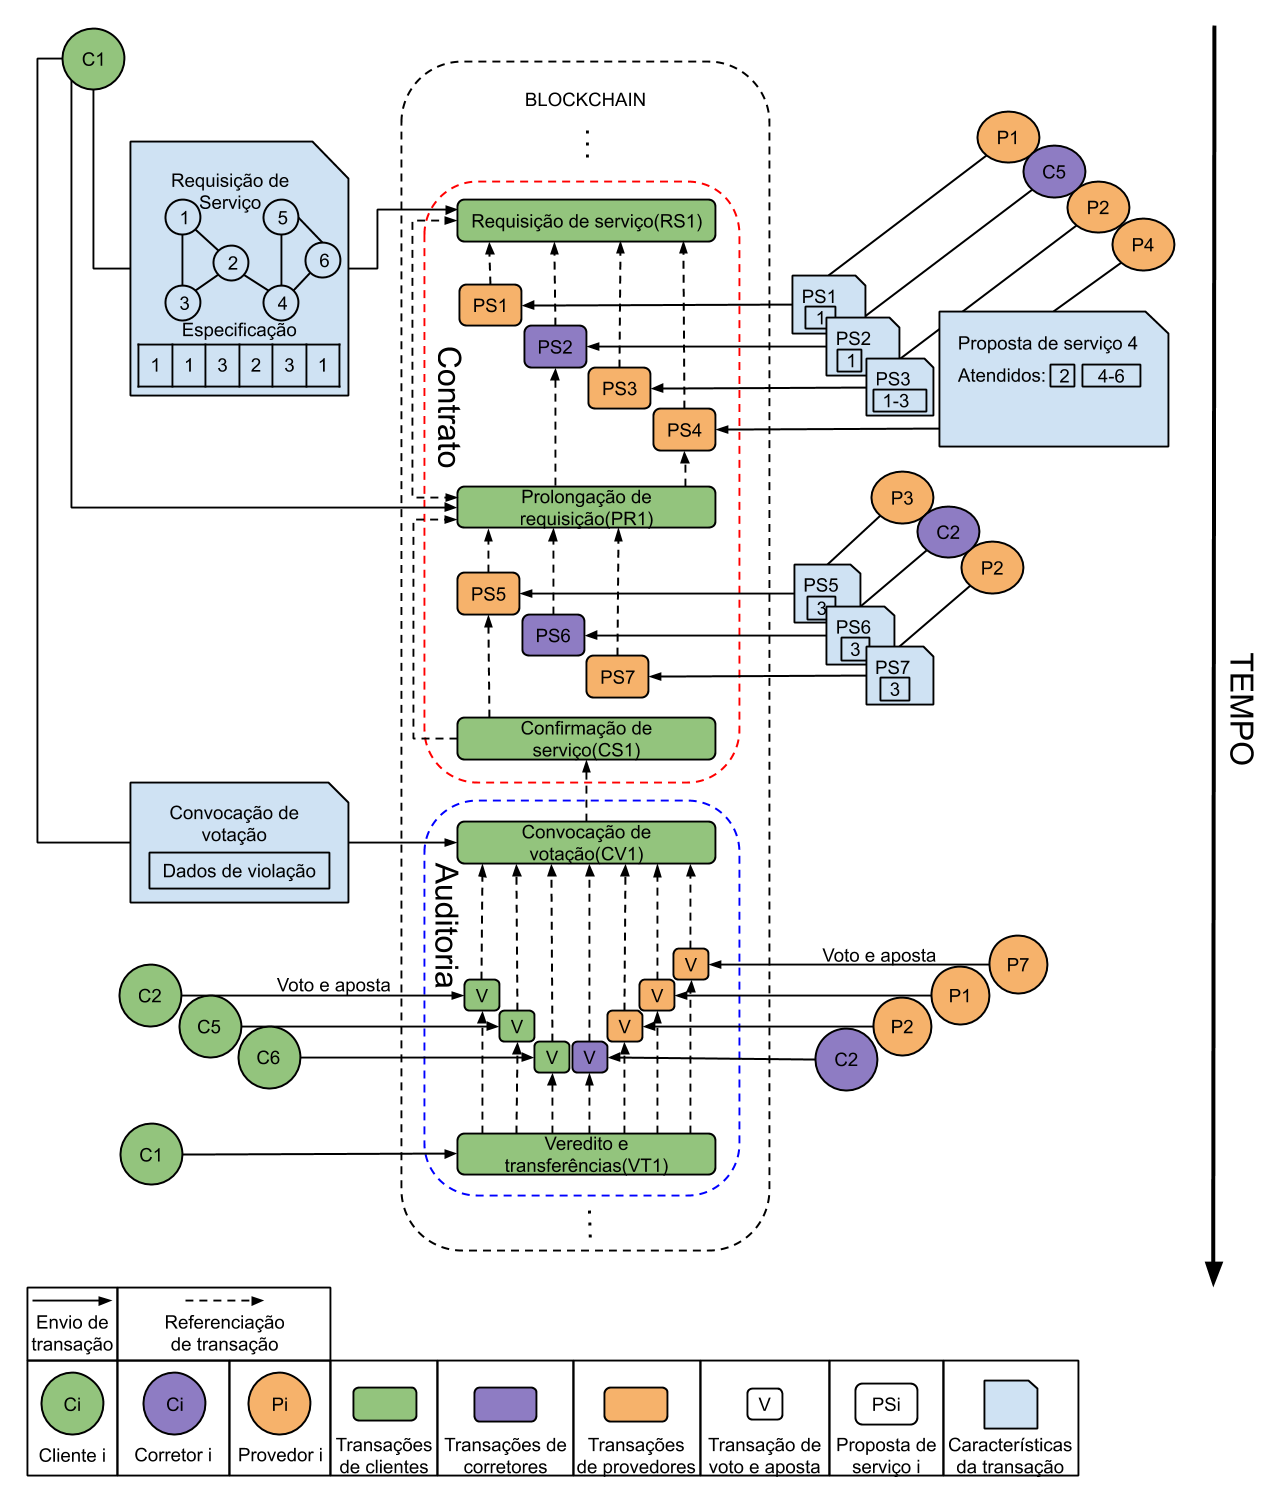
\includegraphics[width=0.96\textwidth]{imagens/cenario_execucao.png}
\begin{center}
        Fonte: Autor.
\end{center}
\label{fig:cenario_execucao}
\end{figure}


Clientes envolvidos no processo são representados por círculos verdes e por uma legenda contendo a letra maiúscula C, bem como um índice numérico referente ao cliente em questão. O mesmo vale para os provedores, que além de serem reconhecidos pelos índices individuais, são representados por círculos laranjas e pela letra P. Os corretores de forma semelhante são representados por círculos roxos com a letra C. A diferenciação entre provedores e corretores é aqui empregada apenas para fins ilustrativos, porém como abordado na Seção \ref{sec:proposta:atores} não há diferenças entre seus papéis práticos. A cadeia de blocos é representada por um retângulo tracejado e referenciações para transações passadas são identificadas através de flechas tracejadas em direção à transação pai. Envios de transações para a rede por parte dos atores são representados por flechas contínuas que iniciam no ator e terminam dentro da \textit{Blockchain}. Detalhes importantes das transações enviadas são mostrados através de retângulos azuis no meio das flechas de envio. Transações de autoria de usuários na cadeia são coloridas de acordo com a cor referente ao tipo do mesmo. 

% Outras Informações específicas a respeito da estrutura das transações e funcionamento de baixo nível do sistema serão explicadas no decorrer da se Seção.

\section{Fase Contratual}
\label{sec:proposta:fase_contratual}

A fase contratual representa o início de um ciclo completo do protocolo e compreende todo o processo relativo ao estabelecimento de um contrato e as negociações realizadas para tal. Essa fase é representada na Figura \ref{fig:cenario_execucao} por um retângulo tracejado vermelho com a legenda "Contrato".


\subsection{Requisições de Serviço}
\label{subsec:proposta:contratual:rs}
%
Os contratos na rede proposta devem ser atômicos, assim não é possível fechar um contrato sem que todos os microsserviços elencados pelo cliente sejam devidamente supridos pela infraestrutura de algum prestador de serviço. Após a entrada de um usuário na rede este já está apto a estabelecer contratos com provedores, o primeiro passo para realizar esse processo é a escrita de uma nova transação, que representa uma requisição de serviço. Essa requisição de serviço descreve um conjunto de microsserviços que, como pode ser observado na Figura \ref{fig:cenario_execucao}, são organizados em um grafo não direcionado, de forma que os nós representam os microsserviços em si e as arestas os enlaces necessários para que a comunicação seja realizada corretamente. Junto ao grafo encontra-se um vetor com tamanho igual à quantidade de microsserviços, cujo valor de cada célula $i$ representa o índice da função - no caso de \ac{FaaS} - ou infraestrutura  requerida para o microsserviço respectivo.


Ainda junto a \ac{RS} devem estar definidas todas as infraestruturas ou funções referenciadas pelos índices contidos no vetor para que seja possível a interpretação por parte dos prestadores de serviço. Para implementar tal aspecto arquitetural será utilizada uma linguagem de definição de infraestrutura de modo a padronizar os dados contidos nas requisições. Métodos de \ac{IasC} baseados em linguagens de definição são empregados em certas tecnologias de nuvem para agilizar e automatizar o processo de implantação das infraestruturas virtuais. A \textit{Amazon} por exemplo, utiliza o \textit{CloudFormation} \cite{nuvem_sla:cloudformation}, que permite aos usuários escrever \textit{scripts} completos ou utilizar \textit{templates} de infraestruturas comuns para implantar e atualizar os serviços contratados. O \textit{OpenStack} faz uso do \textit{Heat} \cite{nuvem_sla:heat}, que de forma semelhante ao anterior, utiliza \textit{templates} para garantir a alocação correta e eficiente das infraestruturas de maneira automatizada.
VXDL, por sua vez, permite a descrição completa da infrastrutura, incluindo os requisições de comunicação~\cite{nuvem_sla:vxdl}.

%
A Tabela \ref{tabela:rs} mostra todos os campos que compõem a transação de requisição de serviço exclusivamente, uma breve descrição para suas respectivas funções e o tamanho em \textit{bytes} para cada um. Essa transação também possui os campos comuns listados na Seção \ref{tabela:dados_comuns}.
\begin{table}[ht]
\centering
    \begin{tabular}{|m{0.15\textwidth}|m{0.6\textwidth}|m{0.15\textwidth}|}
    \hline
         \textbf{Campo} & \textbf{Descrição} & \textbf{Tamanho}  \\
         \hline
         Tamanho dos dados & Indica o tamanho em \textit{bytes} dos dados da requisição & 4 \textit{bytes} \\
         \hline
         Dados & Armazena os dados referentes às infraestruturas ou funções necessárias para o serviço em questão & Variável \\
    \hline
    \end{tabular}
    \caption{Campos da transação de Requisição de Serviço}
    \label{tabela:rs}
\end{table}

O primeiro campo da Tabela~\ref{tabela:rs} indica o tamanho dos dados ou carga propriamente dita da transação que vem em seguida. O segundo campo armazena os dados em si utilizados para descrever as infraestruturas ou funções requeridas e suas relações com os microsserviços necessários. 

A escolha de uma seção abstrata de dados ao invés de campos individuais para representar estruturalmente um grafo com os dados é tomada com vista na adaptabilidade do protocolo. Assim, a modularização da proposta é reforçada e novas formas de representação das informações relevantes para o contrato podem ser empregadas através do versionamento da transação. Modificações nas estruturas de dados podem ser motivadas por diversos fatores, tais como adição de novas características para infraestruturas, novas definições de \ac{FaaS}, melhor detalhamento das infraestruturas, \textit{etc}.

O protocolo em sua parte majoritária funciona de maneira agnóstica à forma da representação e armazenamento dos dados, porém o processo de validação da transação necessita acesso aos dados e portanto deve conhecer seus formatos para garantir características básicas de coesão da requisição como conectividade e coerência das conexões. Assim o fluxograma que representa os processos necessários para que a transação de \ac{RS} seja aceita é mostrado na Figura \ref{fig:validacao_rs}.

\begin{figure}[ht!]
\caption{Fluxograma para validação de uma Requisição de Serviço.}
\centering
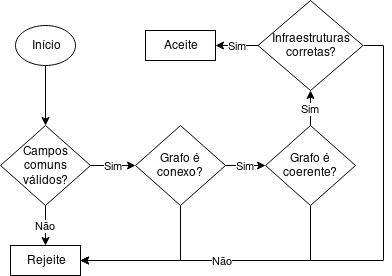
\includegraphics[width=0.75\textwidth]{imagens/validacao_rs.png}
\begin{center}
        Fonte: Autor.
\end{center}
\label{fig:validacao_rs}
\end{figure}

Primeiramente são validados os campos comuns e uma vez que sua validade é atestada parte-se para os dados do grafo em si. O grafo deve ser conexo para que então seja verificada a coerência do mesmo. O conceito de coerência dos dados envolve a verificação de que todas as arestas partem de um nó valido e chegam a outro nó válido e que não há nenhum par de nós $x$ e $y$ com mais de uma aresta entre eles. Por fim, a verificação das infraestruturas garante que cada microsserviço listado no grafo possui uma infraestrutura relativa e que tais infraestruturas estão corretamente definidas na sintaxe de representação. 

Por fim, há uma quantidade finita de requisições de serviço abertas que um usuário pode ter em um determinado momento, de modo que quando esse limite é atingido é necessário fechar contratos - se todos os microsserviços foram atendidos com infraestruturas correspondentes - ou finalizá-las para que a criação de novas requisições seja liberada. Transações de \ac{RS} têm referenciação permitida para o usuário criador através das transações de \ac{PR} e \ac{CS} e para o grupo de prestadores de serviço através da transação de \ac{PS}.

% \subsection{Definições de infraestrutura}
% \label{subsec:proposta:contratual:di}
% %
% Diferentes microsserviços de uma mesma requisição podem ter necessidades diferentes de infraestrutura e portanto as transações de \ac{RS} devem referenciar outras transações chamadas \ac{DI}, que podem ou não ser escritas pelo usuário que faz a requisição. Na rede, qualquer participante pode escrever um número finito de transações de \ac{DI} e estas podem ser referenciadas por qualquer outro usuário que deseja fazer uma requisição. Assim sendo, provedores podem publicar definições padrão que costumam oferecer, como se fossem planos predefinidos de serviço, enquanto usuários podem criar novas definições para microsserviços com necessidades específicas que podem, eventualmente, servir para outros usuários em condições semelhantes. Atualizações nas definições podem ser feitas pelos criadores em caso da necessidade de adaptação de infraestruturas para novos contratos, sendo representadas por uma nova \ac{DI} que referencia a anterior. Novas versões de \acp{DI} apenas podem ser criadas caso já exista algum contrato firmado que as referenciem, para evitar o surgimento de definições órfãs ou o superpovoamento de definições pelos usuários. Portanto, usuários podem ter um número finito predeterminado de definições existentes sem referenciação e nada impede o criador ou outros clientes de referenciar versões passadas de uma \ac{DI}. 

% Para que seja possível realizar tal aspecto arquitetural será utilizada uma linguagem de definição de infraestrutura que representa os dados em si carregados pela \ac{DI}. Métodos de \ac{IasC} baseados em linguagens de definição são empregados em certas tecnologias de nuvem para agilizar e automatizar o processo de implantação das infraestruturas virtuais. A \textit{Amazon} por exemplo, utiliza o \textit{CloudFormation} \cite{nuvem_sla:cloudformation}, que permite aos usuários escrever \textit{scripts} completos ou utilizar \textit{templates} de infraestruturas comuns para implantar e atualizar os serviços contratados. O \textit{OpenStack} faz uso do \textit{Heat} \cite{nuvem_sla:heat}, que de forma semelhante ao anterior, utiliza \textit{templates} para garantir a alocação correta e eficiente das infraestruturas de maneira automatizada.

% O objetivo dessa escolha de arquitetura é primeiramente reduzir a duplicação de informação, uma vez que muitos clientes podem querer utilizar arquiteturas idênticas, cujas diferentes requisições de serviço não precisam reter as informações consigo, mas apenas referenciá-las. Consequentemente, as dificuldades de escalabilidade da rede se tornam mais brandas, devido ao menor volume de dados que é preciso armazenar em todos os dispositivos conectados. Esse tipo de abordagem leva à consequente formação de uma biblioteca pública de definições de infraestruturas virtuais, na qual usuários publicam informações e utilizam as de terceiros. Um exemplo do funcionamento de uma ideia semelhante é o \textit{Docker Hub} \cite{nuvem_sla:docker_hub}, que trata-se de um repositório de compartilhamento público de imagens de contêineres administrado pelo \textit{Docker}. Através dessa plataforma usuários podem baixar \textit{templates} publicados por outros participantes ou criar e disponibilizar os seus próprios para o uso da comunidade em geral, criando oportunidade de utilização de inúmeras imagens já preparadas.

\subsection{Prolongação de Requisição}
\label{subsec:proposta:contratual:pr}
%
Um cliente, após abrir uma requisição, pode esperar propostas de serviço por tempo indeterminado até encontrar as que mais se adéquem às suas preferências. Ocasionalmente, o aparecimento de novas propostas para uma requisição cessa, decorrente do envelhecimento da transação em questão na cadeia, que acarreta em baixa visibilidade para outros provedores. Outro possível cenário trata-se do cliente se interessar por propostas que contemplam apenas uma parcela dos microsserviços, mas não por aquelas que contemplam outra, da mesma forma que a requisição pode não receber propostas suficientes para abranger os microsserviços em completude. Na ocorrência de tais casos, o usuário pode criar uma \ac{PR} que serve para explicitar quais das propostas feitas até o momento foram escolhidas para a requisição, sendo indicadas através da referenciação das transações das \acp{PS}. Similarmente, se nenhuma das propostas feitas até então para a \ac{RS} for de interesse do cliente, nada impede-o de criar uma \ac{PR} sem nenhuma referenciação para propostas existentes.

%
Após a criação dessa transação, o efeito gerado na rede é o reavivamento da requisição, que acontece devido a transmissão da \ac{PR} como uma nova transação, atraindo o olhar de prestadores de serviço. Nessa transação, além dos campos comuns mencionados na Seção \ref{subsec:campos_comuns} são necessários os campos mostrados na tabela \ref{tabela:pr}.

\begin{table}[ht]
\centering
    \begin{tabular}{|m{0.15\textwidth}|m{0.6\textwidth}|m{0.15\textwidth}|}
    \hline
         \textbf{Campo} & \textbf{Descrição} & \textbf{Tamanho}  \\
         \hline
         \ac{RS} \textit{Hash} & Contém o \textit{Hash} criptográfico da \ac{RS} sendo referenciada e serve como apontador na cadeia & 32 \textit{bytes} \\
         \hline
         Quantidade de propostas & Indica o total de propostas aceitas até o momento para a \ac{RS} & 4 \textit{bytes} \\
         \hline
         \textit{Hashs} \acp{PS} & Vetor com os \textit{hashs} de todas as propostas aceitas & Variável \textit{bytes} \\
    \hline
    \end{tabular}
    \caption{Campos da transação de Prolongação de Requisição}
    \label{tabela:pr}
\end{table}

O primeiro campo da Tabela~\ref{tabela:pr} se refere ao \textit{hash} da \ac{RS} ao qual se pretende prolongar e naturalmente deve ser de criação do mesmo usuário que criou a \ac{PR} em questão. O segundo campo trata-se da quantidade de propostas que foram aceitas pelo usuário e existe para propósitos de serialização. O terceiro campo trata-se de um vetor de tamanho igual ao segundo campo e contém os \textit{hashs} de todas as transações de Proposta de Serviço registradas na cadeia cujas quais se pretende aceitar através da transação atual em questão. A validação de \acp{PR} segue de acordo com o fluxograma mostrado na Figura \ref{fig:validacao_pr}.

\begin{figure}[ht!]
\caption{Fluxograma para validação de uma Prolongação de Requisição.}
\centering
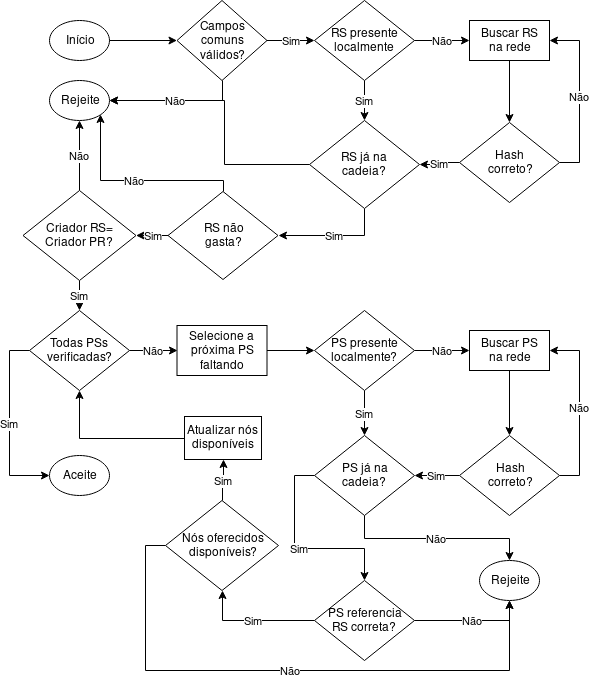
\includegraphics[width=0.8\textwidth]{imagens/validacao_pr.png}
\begin{center}
        Fonte: Autor.
\end{center}
\label{fig:validacao_pr}
\end{figure}

Primeiramente são validados os campos comuns e é recuperada a transação de \ac{RS} original, sua correta inserção na cadeia e disponibilidade de referenciação também são checadas. Verifica-se então que ambas as transações possuem o mesmo criador e que todas as propostas estão corretas, que já pertencem à cadeia e que os serviços oferecidos por elas não suprem nós que não estão mais disponíveis. Se todas essas suposições forem consideradas verdadeiras ao final do processo a transação é tida como válida.   

% \begin{enumerate}
%     \item Verificar os campos comuns.
%     \item Verificar se o tipo informado nos campos comuns. condiz com os dados seguintes da transação.
%     \item Verificar que a presença local da transação de \ac{RS} referenciada. Caso não esteja presente a transação deve ser requisitada da rede.
%     \item Verificar que o endereço listado como criador da transação é o mesmo da transação de \ac{RS}.
%     \item
% \end{enumerate}

%
Novas \ac{PS} podem então ser feitas por parte dos prestadores de serviço, agora referenciando não a requisição original, mas sim a prolongação de requisição relacionada, buscando assim finalizar o processo de escolha dos serviços. A quantidade de \ac{PR} que uma requisição pode ter é limitada, pois pode ocorrer de que certos microsserviços apenas não sejam mercadologicamente viáveis para o atendimento dos prestadores. Em face de tal ocorrido, a única alternativa é recomeçar o processo criando uma requisição em que as características dos microsserviços não atendidos sejam modificadas. Entretanto, presume-se que o aparecimento do referido cenário é esparso e que a maioria das requisições são completamente atendidas. A transação de Prolongação de Requisição pode ser referenciada por qualquer prestador de serviço através da transação de Proposta de Serviço e pelo usuário criador por uma Confirmação de Serviço.

%
\acresetall
\subsection{Propostas de Serviço}
\label{subsec:proposta:contratual:PS}

Após a escrita de uma \ac{RS} ou \ac{PR} na cadeia, propostas de serviço podem ser enviadas para suprir tal demanda. Provedores e corretores podem referenciar a requisição em questão criando novas transações chamadas \ac{PS}, que contém uma oferta da infraestrutura desejada para um ou mais microsserviços. Uma vez que grande parte das informações a respeito da alocação em si já foram definidas na \ac{RS} sendo referenciada, \acp{PS} não possuem grandes cargas de dados e a principal informação contida em tal forma de transação é o preço para o qual o provedor se dispõem a realizar o serviço descrito na proposta. \acp{PS} podem ser usadas para responder qualquer \ac{RS} ou \ac{PR} desde que originada de um usuário pertencente aos grupos permitidos.
%

Assim como na transação de \ac{RS} esta forma possui todos os campos comuns mencionados na Seção \ref{tabela:dados_comuns} e ainda campos individuais próprios descritos na tabela \ref{tabela:ps}.

\begin{table}[ht]
\centering
    \begin{tabular}{|m{0.15\textwidth}|m{0.6\textwidth}|m{0.15\textwidth}|}
    \hline
         \textbf{Campo} & \textbf{Descrição} & \textbf{Tamanho}  \\
         \hline
         \acs{PC} \textit{Hash} & Contém o \textit{hash} criptográfico da transação de publicação do certificado referente ao prestador de serviço & 32 \textit{bytes} \\
         \hline
         \ac{RS}/\acs{PR} \textit{Hash} & Contém o \textit{hash} criptográfico da \ac{RS} ou \acs{PR} sendo referenciada e serve como apontador na cadeia & 32 \textit{bytes} \\
         \hline
         Semente criptografada & Indica um valor aleatório criptografado escolhido pelo provedor & 32 \textit{byte} \\
         \hline
         Política de preço & Indica de qual forma será feita a cobrança pelo serviço através de um código predefinido & 1 \textit{byte} \\
         \hline
         Preço & Contém o preço a ser cobrado de acordo com a política de precificação escolhida & 4 \textit{byte} \\
         \hline
         Quantidade de nós & Indica a quantidade de nós do grafo da \ac{RS} que essa proposta pretende atender & 4 \textit{bytes} \\
         \hline
         Nós atendidos & Contém o índice de todos os nós atendidos no grafo da \ac{RS} sendo referenciada & Variável \\
    \hline
    \end{tabular}
    \caption{Campos da transação de Proposta de Serviço}
    \label{tabela:ps}
\end{table}

O segundo campo da Tabela~\ref{tabela:ps} contém o \textit{hash} da Requisição de Serviço ou Prolongação de Requisição já presente na cadeia ao qual essa proposta é destinada. O terceiro campo tem seu uso destinado ao posterior processo de votação e interpretação dos dados de monitoração coletados, os detalhes a respeito de sua aplicação são descritos na Seção \ref{subsec:proposta:votacao_detalhada}.

%
O quarto campo indica qual será a política de preço adotada ou de forma geral, de que maneira se dará a cobrança pelos serviços prestados, sendo estas representadas por um código numérico de um \textit{byte}, que pode assumir 256 diferentes valores. O quinto campo é destinado ao preço que será cobrado de acordo com a política especificada no terceiro campo e seu valor corresponde a um ponto flutuante de quatro bytes de acordo com o padrão IEEE 754 \cite{nuvem_sla:padrao_i3e}. O sexto campo é a quantidade de nós relativos a \ac{RS} que a proposta pretende atender, que serve para a correta serialização e desserialização da transação e deve ser obrigatoriamente menor ou igual a quantidade de nós presentes na respectiva \ac{RS}. O sétimo e último campo trata-se de um vetor de inteiros do tamanho descrito no quinto campo, este deve conter os índices dos nós atendidos por essa proposta na referente requisição do cliente. Nesse caso, embora a definição do grafo com as informações de alocação seja originalmente representada de maneira abstrata, acredita-se que independentemente da forma escolhida haverá inevitavelmente uma ordenação lógica para os nós e arestas que pode ser acessada através de índices numéricos como realizado nesse campo. A Figura \ref{fig:validacao_ps} contém o fluxograma básico para a validação de propostas de serviço.

\begin{figure}[ht!]
\caption{Fluxograma para validação de uma Proposta de Serviço.}
\centering
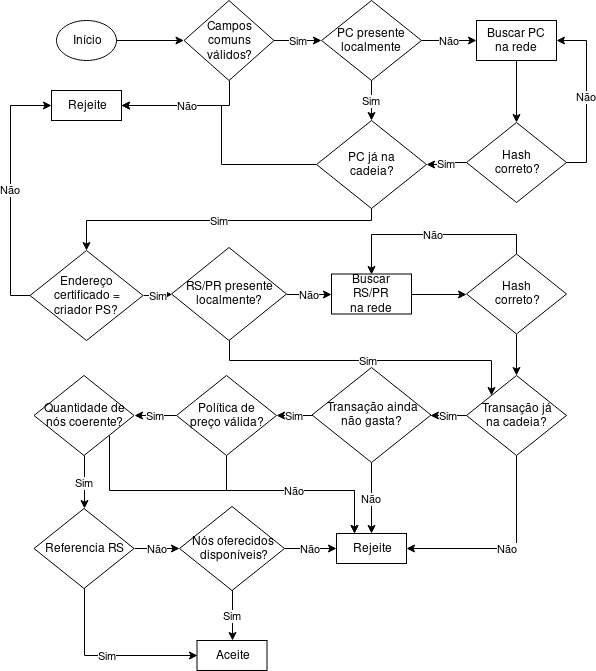
\includegraphics[width=0.8\textwidth]{imagens/validacao_ps.png}
\begin{center}
        Fonte: Autor.
\end{center}
\label{fig:validacao_ps}
\end{figure}

Os campos comuns são verificados primeiramente e em seguida recupera-se a transação que contém o certificado do prestador de serviço para que sua identidade possa ser atestada. Recupera-se também a transação de \ac{RS} ou \ac{PS} sendo referenciada e verifica-se se ela ainda pode ser respondida. No caso de se tratar de uma prolongação de requisição os nós atendidos são verificados para evitar conflito com propostas já aceitas. Se algum dos passos de verificação não for completamente verificado e resultar em fracasso, a transação é considerada inválida. Para esta transação, a referenciação é permitida apenas para o criador da requisição de serviço cuja a proposta pretende atender.

\subsection{Confirmação de Serviço}
\label{subsec:proposta:contratual:cs}

O último processo da fase contratual é a \ac{CS}, nela o usuário cria uma transação que deve referenciar as propostas de serviço restantes da última \ac{PR} ou, no caso de não houver nenhuma, a \ac{RS} original. Essa transação é de suma importância pois é responsável por selar o contrato de \ac{IaaS} com todos os provedores e suas \acp{PS} selecionadas no processo até então. A partir da existência de uma \ac{CS} na cadeia, nenhuma nova proposta de serviço que referencia a requisição ou prolongações dessa \ac{CS} passa no processo de validação por qualquer nó. A alocação das infraestruturas oficializadas pelo protocolo não é regida nem supervisionada por ele, porém acredita-se que nenhum dos atores envolvidos têm motivos para não realizá-la no mundo real, pois o prestador do serviço quer vender o produto (\textit{i.e.}, obter lucro) e o cliente quer sua aplicação funcionando no mercado. Mesmo em casos esdrúxulos nos quais por algum motivo a alocação não ocorra de verdade, esse contrato não afeta o futuro da rede, porque o voto em acusações contra qualquer um dos provedores envolvidos depende das provas criptográficas de monitoração, que invariavelmente não existirão sem a alocação física. A tabela \ref{tabela:cs} mostra todos os campos individuais utilizados por esse tipo de transação e suas definições. 

\begin{table}[ht]
\centering
    \begin{tabular}{|m{0.15\textwidth}|m{0.6\textwidth}|m{0.15\textwidth}|}
    \hline
         \textbf{Campo} & \textbf{Descrição} & \textbf{Tamanho}  \\
         \hline
         \ac{RS}/\ac{PR} \textit{Hash} & Contém o \textit{Hash} criptográfico da \ac{RS} ou \ac{PR} sendo referenciada para fechar o contrato & 32 \textit{bytes} \\
         \hline
         Quantidade de propostas & Indica o total de propostas aceitas até o momento para a \ac{RS} & 4 \textit{bytes} \\
         \hline
         \textit{Hashs} \acp{PS} & Vetor com os \textit{hashs} de todas as propostas aceitas & Variável \textit{bytes} \\
    \hline
    \end{tabular}
    \caption{Campos da transação de Confirmação de Serviço}
    \label{tabela:cs}
\end{table}

O primeiro campo dessa transação trata-se do \textit{hash} criptográfico tido como apontador na cadeia, referenciando uma requisição de serviço ou prolongação de requisição e indicando o fechamento do respectivo contrato estipulado por tais transações. O segundo campo indica a quantidade de propostas que serão aceitas para a finalização o contrato, servindo para fins de serialização. O terceiro campo compreende um vetor com os \textit{hashes} de todas as \acp{PS} que serão contratadas, de modo que os nós que estas suprem, unidos com os nós supridos por todas as \acp{PS} referenciadas por eventuais \acp{PR} devem compreender todo o grafo de infraestruturas. O processo de validação de uma transação de Confirmação de Serviço se dá de acordo com o fluxograma mostrado na Figura \ref{fig:validacao_cs}.

\begin{figure}[ht!]
\caption{Fluxograma para validação de uma Confirmação de Serviço.}
\centering
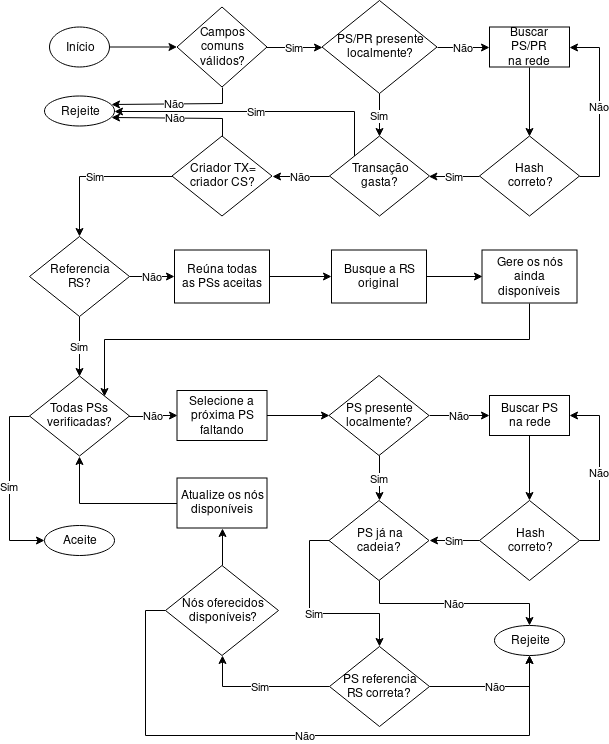
\includegraphics[width=0.8\textwidth]{imagens/validacao_cs.png}
\begin{center}
        Fonte: Autor.
\end{center}
\label{fig:validacao_cs}
\end{figure}

Outra vez inicia-se a verificação pelos campos comuns e se esses estiverem corretos busca-se a transação que está sendo referenciada, garantindo também que o seu criador e o da transação atual são o mesmo. No caso da referência à uma \ac{RS}, apenas são buscadas todas as propostas referenciadas e verificada a inexistência de conflitos nos nós atendidos. O processo é semelhante para o caso da \acp{PR}, porém antes de serem verificadas as novas propostas referenciadas cria-se uma lista de nós ainda disponíveis a partir das propostas já aceitas anteriormente. Assim se não houver conflito no atendimento das propostas e todas as outras verificações foram feitas com sucesso, a transação é validada.
%
Após a criação e validação de uma confirmação de serviço, já é possível que a fase de auditoria seja iniciada.

\section{Fase de Auditoria}
\label{sec:proposta:fase_auditoria}
\acresetall

A fase de auditoria ocorre quando um usuário detecta que seu contrato foi violado pelo provedor e medidas para auditoria da ocorrência de quebra ou não, são então tomadas pela rede. Essa fase é representada por um retângulo tracejado azul com a legenda "Auditoria" na Figura \ref{fig:cenario_execucao}. Essa fase baseia-se em dois pilares fundamentais, sendo o primeiro o contrato estabelecido e os dados do mesmo existentes na \textit{Blockchain} e o segundo um conjunto de dados relativos à execução da alocação, coletados por um módulo de monitoração auxiliar da carteira.
%
Usuários clientes monitoram exclusivamente provedores com os quais possuem algum contrato firmado, ao passo que usuários prestadores de serviço podem - e é de seus interesses - monitorar outros usuários do mesmo grupo.

%
A inter-monitoração de prestadores de serviço ocorre de maneira paralela à cadeia, assim dados recolhidos são mantidos localmente pelo realizador do processo e fornecidos aos outros usuários apenas como comprovação de voto no momento apropriado. Esses dados, embora possuam um dono teórico e sejam eventualmente compartilhados, não devem ser interpretáveis por nenhum ator que não a carteira digital em si de cada usuário. Dessa forma, mesmo o agente externo à rede que possui controle sobre a carteira não consegue entender os dados que produz ou recebe, sendo que a coerência empírica desses apenas existe no contexto de execução da carteira, que é alheio ao usuário.

%
Um processo significativo que acontece na fase de auditoria é a movimentação e redistribuição de pontos de reputação. Esse fenômeno acontece pois todos os usuários que desejam participar do processo de votação a respeito de um contrato devem apostar uma parte de suas reputações, de modo a garantir respaldo para os dados que estão sendo enviados para a avaliação coletiva, o que significa que os votantes apostam na veracidade e precisão das suas monitorações. A aposta possui um valor mínimo requerido mas não um valor máximo, portanto cabe ao usuário decidir quanto deseja alienar ao processo e naturalmente, apostas maiores conferem maiores prêmios em caso de assertividade.

\subsection{Módulo de Monitoração}
\label{sec:proposta:monitoracao}

O módulo de monitoração é um dos grandes componentes da rede e existe como um apêndice da carteira de cada usuário, devendo ser alocado junto a infraestrutura contratada pelo cliente para realizar o processo de monitoração. A coleta dos dados é feita através de um processo de estresse na infraestrutura, que busca levá-la a utilização máxima de seus recursos para atestar a entrega completa do acordado em contrato. A periodicidade das monitorações é definida de maneira prévia e todos os módulos operam na mesma frequência, garantindo assim que a diferença temporal máxima entre as últimas monitorações de dois módulos distintos é sempre menor ou igual a um período. Portanto, se por exemplo a frequência de monitoração é de um teste a cada 10 minutos, naturalmente a diferença máxima entre as últimas monitorações de dois usuários distintos pode ser de, no máximo, 10 minutos.

%
% No que diz respeito ao intervalo em si, a possibilidade do uso de períodos de tempo muito elevados não possuiria utilidade prática pois os dados resultantes não seriam consistentes. Esse fato se manifesta porque a própria esparsidade dos testes abrangeria frações muito pequenas de utilização dos recursos quando comparadas ao tempo total não monitorado, dificultando a convergência de dados provenientes de diferentes usuários sobre a frequência ou até mesmo ocorrência de quebras. Assim, como com uma periodicidade muito baixa a disparidade nos horários de realização de testes tenderia a ser muito grande, o uso de intervalos curtos na ordem de minutos é correto e deve ser empregado. 

% TODO: não concordo muito com tal discussão. Existe uma linha de pesquisa especifica sobre monitoramento de recursos. Parece perigoso afirmar tal raciocínio sem conhecer a aplicação alvo. A carga da aplicação. Enfim, vamos pensar, mas podemos remover a discussão (parágrafo anterior).

%
A primeira vista, a comparação de monitorações realizadas em dispositivos diferentes sem sincronização de relógio pode parecer incoerente, porém com períodos de tempo relativamente pequenos e contextos de monitoração presumidamente semelhantes em casos de quebra de contrato, como apontado na Seção \ref{sec:proposta:definicoes}, é bastante improvável que violações não sejam detectadas em múltiplos dados de monitoração diferentes.

%
Os dados coletados pelo módulo são guardados localmente na infraestrutura contratada e somente são enviados para a carteira ou de forma geral ao dono dos mesmos mediante uma requisição explícita para tal. O módulo possui um par de chaves assimétricas privada e pública, sendo a chave privada igual para todos os módulos de todos usuários e podendo ser armazenada em algum local do código fonte ou construída secretamente dentro de um sistema de enclaves criptográficos. O propósito e utilização do par de chaves do módulo é garantir a confidencialidade das informações mantidas por ele localmente, que são criptografadas utilizando-se de sua chave pública. Assim, mesmo que os dados sejam descobertos ou copiados do disco, o atacante ou invasor não conseguiria ver o texto em claro devido à falta da chave privada, que é conhecida apenas pelo módulo em sua execução. O par de chaves ainda possui outros usos que são apresentados na Subseção \ref{subsec:proposta:votacao_detalhada}.

% TODO: você indicou uma divisão em arquivos. Mas seria uma proposta de implementação, certo? Não é relacionado com a rede em si. Podemos simplificar?

%
Internamente, o módulo armazena todos os dados de monitoração colhidos durante um determinado período preestabelecido, sejam eles comprobatórios ou não de ocasionais quebras. Os dados armazenados devem conter um registro individual de cada teste, de modo a evitar o uso repetido de monitorações já utilizados em uma votação e naturalmente um valor de porcentagem para aquele aspecto, indicando se o fornecimento foi adequado ou não.

% A organização é dividida em arquivos, de modo que cada um dos possíveis componentes suscetíveis à violação como quantidade de RAM, processamento, vazão, \textit{jitter}, \textit{etc}, sejam indexados em um arquivo individualizado. Dentro de cada arquivo há uma série de linhas de dados que resumem o histórico dos resultados de testes individuais para aquela categoria. Uma linha é composta por:
% \begin{itemize}
    % \item Um número de série ou índice, que deve obrigatoriamente ser maior que o da linha anterior e menor que o da linha seguinte, servindo como indicação de que não houve alteração ou adição indevida de testes na linha do tempo.
    % \item Um valor normalizado em porcentagem que indica o resultado do teste em si, de modo que ao atingir números próximos de 100\% considera-se que não houveram violações do acordado e ao atingir números inferiores, considera-se que houveram violações cuja gravidade é proporcional ao quão próximo de 0\% o resultado chegou.
% \end{itemize}

Para que o usuário saiba quando houve uma quebra de contrato em sua infraestrutura e possa iniciar uma votação, o módulo é capaz de enviar alertas que indicam qual dos aspectos da infraestrutura foram violados, porém sem especificar qual a porcentagem exata ou a frequência relacionada a essa violação. O mecanismo de alerta binário ao invés de multivalorado é empregado para amenizar a possibilidade de que o usuário dono dos dados possa visualizar os mesmos e divulgá-los a outros participantes. Essa ação por si só não representaria um problema ou vulnerabilidade de segurança, mas poderia contribuir para a prática de outros ataques prejudiciais ao protocolo. Também é importante salientar que objetivando o não surgimento de todo um novo conjunto de problemas de comunicação e concorrência, os módulos operam segundo uma diretiva \textit{standalone} sem troca de informações entre si e o envio de alertas e dados ao usuário são as únicas ações desempenhadas que envolvem comunicação com qualquer contexto externo à infraestrutura sob vigilância. 

%
Quando o envio dos dados é requisitado pelo usuário o módulo não simplesmente transmite os dados criptografados por sua chave pública para o dono, pois embora o objetivo da não descoberta dos dados para compartilhamento prematuro seja garantido, também não seria possível que nenhum usuário participante do processo de votação visualizasse esses dados em nenhum momento, inviabilizando o procedimento como um todo. Para evitar esse problema e ainda garantir a não descoberta utiliza-se uma espécie de chave de sessão - intitulada "chave de votação" a partir do presente momento pela maior proximidade do termo com o uso real no protocolo - para criptografar os dados para envio. Além do conteúdo dos arquivos de um aspecto, adiciona-se à mensagem o \textit{hash} de uma série de informações pertinentes da infraestrutura em que o módulo está sendo executado, isso com o objetivo de garantir a efetividade das provas de monitoração, impedindo que usuários enviem votos com dados provenientes de infraestruturas diferentes das quais as votações foram convocadas e impossibilitar a forja de dados em máquinas inferiores. O processo completo e detalhado de construção dos dados, criação da chave de votação, tradução para envio e visualização conjunta pelos usuários para o veredito é abordado na Seção \ref{subsec:proposta:votacao_detalhada}.

É importante ressaltar que a implementação do módulo de monitoração está além do escopo do presente trabalho, sendo considerado um pré-requisito para a execução do protocolo.
Por fim, Alvorada pode atuar em conjunto com qualquer módulo de monitoração eventualmente disponível.

\subsection{Chaves de Votação}
\label{subsec:chaves_votacao}

Como já mencionado nesta seção os dados coletados pelo módulo de monitoração de um usuário não devem ser visíveis aos outros participantes antes que períodos relativamente avançados da votação sejam atingidos ou esta seja finalizada. Essa medida evita o compartilhamento de informações relevantes, que podem criar meios para um processo de emulação de dados nocivos ao veredito. A finalidade do par de chaves de votação é justamente contornar esse problema, assim o módulo utiliza a respectiva chave privada para traduzir os dados armazenados para uma versão criptografada que seja posteriormente visualizável por todos os participantes. 

%
Para que seja possível um consenso coletivo sobre esses conjuntos de dados claros de diferentes usuários em uma votação, as chaves utilizadas para a tradução dos mesmos devem ser iguais, porém como não há comunicação entre diferentes módulos de monitoração um outro artifício deve ser utilizado. A solução derradeira é o uso de sementes aleatórias iguais entre todos os participantes, que tratam-se unicamente de dois campos preenchidos com valores específicos enviados ao módulo. Dessa forma, toda vez que um usuário solicita os dados coletados por seu módulo ele deve informar junto à requisição os valores de semente que serão usados pelo módulo para a construção do par de chaves de votação. Tal semente pode também ser entendida como a escolha da linguagem sobre a qual a votação acontecerá e assim qualquer usuário que possua dados pertinentes para aquele contexto pode utilizar a semente para habilitá-los a participar da votação.

Tanto o primeiro quanto segundo campos tratam-se simplesmente de dois valores aleatórios de 32 \textit{bytes} criptografados individualmente pela chave pública do módulo. O responsável pela geração da primeira parcela da semente deve ser o prestador de serviço e para cada nova proposta de serviço enviada à cadeia deve ser informado também o primeiro valor da semente - portado no segundo campo da transação de \ac{PS} - que será utilizado para a tradução dos dados em futuras votações contra a mesma, caso venha a ser contratada. O segundo campo deve ser informado pelo usuário - portado no quarto campo da \ac{CV} - e garante que os pares de chaves de votação usados em convocações anteriores movidas por aquele usuário não serão repetidos na transação atual ou próximas transações contra um mesmo serviço fornecido, evitando também a disparidade de poderes de conhecimento entre usuários e prestadores de serviço.

%
A geração da chave privada completa é então feita através da descriptografia do primeiro e segundo campos através da chave privada do módulo, possuindo os dois valores em claro o módulo concatena-os e criptografa o novo valor com sua chave privada, assim o valor criptografado resultante será utilizado como chave de votação para criptografar os dados e enviá-los ao usuário. Para construir a chave pública é utilizada multiplicação em curva elíptica da então construída chave privada por um gerador predefinido na curva, como mostrado na subseção \ref{subsec:ecc}.

%
% Uma vez que o usuário obtêm os dados criptografados deve-se também haver uma forma de receber a chave pública quando o momento for correto para que os dados possam ser visualizados. Entretanto, apenas enviar a chave diretamente ao usuário, junto com os dados por exemplo, não seria eficaz e todo o propósito da criptografia em si se perderia. Para tratar dessa questão é utilizado um sistema criptográfico de limiares, ou esquema de limiares. Os esquemas de limiares para compartilhamento de segredos foram propostos por \citeonline{blockchain:secret_sharing} e consistem de uma forma de dividir um segredo numérico em $n$ partes de forma que possuindo qualquer conjunto de $t$ partes contido em $n$ é possível que o segredo seja reconstruído. Contudo, ao possuir qualquer conjunto com quantidade de partes inferior a $t$ não é possível obter informação de nenhum modo sobre o segredo protegido.

% O esquema de limiares funciona com base na noção matemática de que dado um conjunto de pontos distribuídos no espaço com tamanho $p$, existe apenas um polinômio de grau $p - 1$ cuja fórmula satisfaça todos os pontos do conjunto. Assim, para um conjunto de dois pontos haverá uma e apenas uma reta que cruza ambos, para um conjunto de três pontos haverá única e exatamente uma parábola que os satisfaz, para um conjunto de quatro pontos haverá apenas um polinômio de terceiro grau que os cruza. Adicionalmente, possuindo $p$ pontos há infinitos polinômios de grau $p$ cuja fórmula satisfaz todos os elementos e portanto, possuindo um ponto há infinitas retas que o cruzam, possuindo dois pontos, infinitas parábolas e assim por diante.

% %
% Os esquemas de limiares fazem uso dessa propriedade matemática para que seja possível a divisão do segredo em um conjunto de pontos. Inicialmente deve ser definida a quantidade mínima de partes(pontos) necessárias para a reconstrução do segredo, representada por $q$. Em seguida cria-se um polinômio de grau $q - 1$ cuja aplicação a zero ou $f(0)$ deve ser igual ao segredo que pretende-se dividir. Cada participante então recebe um ponto $(x, f(x))$ que representa sua parte ou sombra do segredo como um todo. Para reconstruir o segredo, uma vez que o indivíduo possui $q$ partes, basta reconstruir o polinômio através da interpolação de Lagrange e dos pontos obtidos e aplicá-lo a zero para encontrar o valor numérico escondido\cite{blockchain:secret_sharing}.

% A interpolação de Lagrange utiliza um conjunto de pontos no espaço e constrói um polinômio único que perpassa-os todos, sua construção e formalização não são comportadas pelo escopo do presente trabalho, porém ela é expressa por:

% \begin{equation}
% \label{lagrange}
%     f(x) = \sum_{i = 1}^{t} y_{i} \prod_{j = 1, j \ne i}^{t} \frac{(x - x_j)}{(x_i - x_j)} (mod p)
% \end{equation}

% onde $t$ é a quantidade de pontos necessários, equivalente a quantidade de partes sobre a qual o segredo foi dividido, $y_i$ e $x_i$ são coordenadas dos pontos e $p$ é um número primo grande que define um campo finito, novamente para propósitos de segurança e robustez do sistema. Tanto $t$ quanto $p$ devem ser conhecidos para que a reconstrução seja possível.

% Supõe-se que um indivíduo deseja compartilhar um segredo que possui valor $6$ com outros dois agentes, porém deseja que ambos devam cooperar para que o valor seja descoberto sem que seja possível visualizá-lo individualmente. Para utilizar o esquema de limiar e querendo que sejam necessárias duas partes para reconstrução do segredo deve ser primeiramente criado um polinômio de grau um, cuja avaliação em zero seja igual a seis, por exemplo $f(x) = (5x + 6) mod p$ - no qual número 13 como definição do campo finito é aqui escolhido arbitrariamente. Posteriormente, envia-se um ponto pertencente a reta com qualquer $x$ diferente de zero para cada um dos dois outros indivíduos, como por exemplo $p(3, 8)$ e $p(7, 2)$. Nesse ponto da execução cada um dos destinatários já possui uma sombra da chave, mas nenhum dos dois sozinhos consegue descobrir qual o segredo. Ao compartilharem suas partes individuais cada um pode calcular o segredo utilizando a equação \ref{lagrange} na forma:

% \begin{equation}
%     f(x) = (8L_1(x) + 2L_2(x)) mod 13
% \end{equation}

% onde

% \begin{equation}
%     L_1(x) = \frac{x - 7}{3 - 7} = \frac{x - 7}{-4} - 13m_1,
%     L_2(x) = \frac{x - 3}{7 - 3} = \frac{x - 3}{4} - 13m_2
% \end{equation}

% e assim

% \begin{equation}
%     f(x) = (2x - 14 + x - 3) mod 13
% \end{equation}

% Nota-se aqui que podem ser criadas milhares de partes distintas distribuíveis entre os usuários uma vez que há infinitos pontos sobre qualquer polinômio no espaço, entretanto mesmo com uma quantidade elevada de partes são necessárias


\subsection{Fluxo de Votação Detalhado}
\label{subsec:proposta:votacao_detalhada}

O processo de votação, embora resida majoritariamente na fase de auditoria, certas características importantes para seu funcionamento se expandem também para a fase de contrato, como mostrado na Seção \ref{subsec:chaves_votacao}. Aqui o processo completo de votação envolvendo todas as interações entre diferentes usuários é expressado na Figura \ref{fig:votacao_detalhada}.

\begin{figure}[ht!]
\caption{Fluxo completo do processo de votação.}
\centering
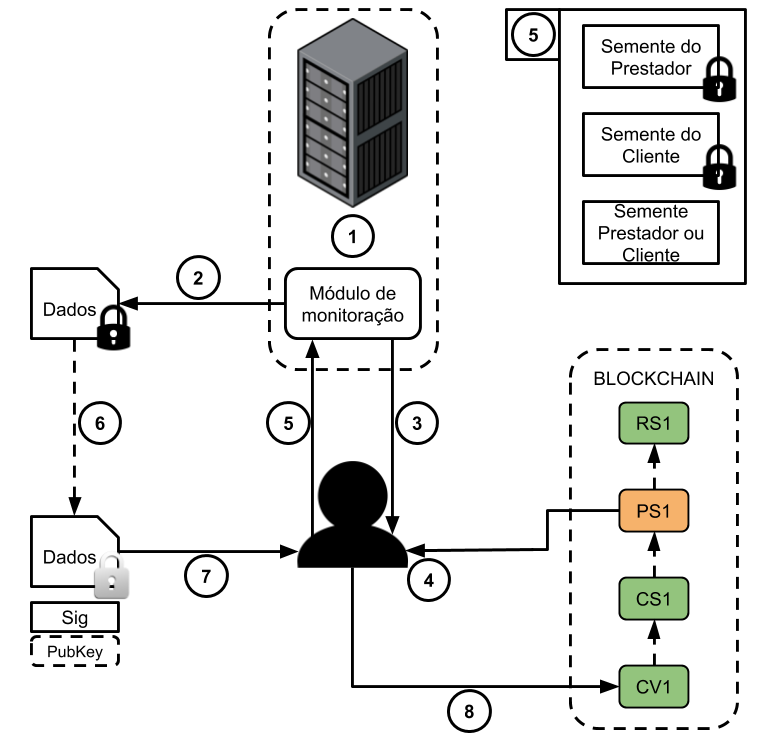
\includegraphics[width=1\textwidth]{imagens/votacao_detalhada.png}
\begin{center}
        Fonte: Autor.
\end{center}
\label{fig:votacao_detalhada}
\end{figure}

Todo o processo específico mostrado diz respeito ao usuário que sofreu a quebra e que está convocando a votação. 

% TODO: indicar que a seta 1 indica uma instalação. Quem sabe colocar um retângulo pontilhado indicando que está executando no servidor.

\begin{enumerate}[label=\textbf{\arabic*})]
    \item Após a confirmação da contratação de um serviço e o fornecimento de acesso aos recursos para o usuário, deve ser inserida uma instância do módulo de monitoração dentro da infraestrutura, naturalmente junto a aplicação específica do cliente.
    \item  À medida que o tempo avança, a cada período de monitoração, o módulo realiza um teste na infraestrutura buscando averiguar a correta disponibilidade dos recursos. Assim que o teste é finalizado, uma nova linha com os dados obtidos é criada para cada arquivo que representa um aspecto passível de violação. Antes de ser anexada ao arquivo, a linha é criptografada utilizando a chave pública do módulo, evitando assim a visualização por parte de agentes externos ou o próprio usuário dono.
    \item Ao executar um certo teste no tempo e notar uma quebra de contrato, o módulo envia ao usuário uma notificação informando a existência de tal quebra e qual aspecto foi negligenciado.
    \item O usuário então, desejando a restituição da quebra deve iniciar uma votação, porém primeiramente é necessário traduzir os dados para uma forma que qualquer usuário possa visualizar após o final da votação. Para tal, o usuário recupera na cadeia a semente criptografada fornecida pelo provedor na \ac{PS} contratada e cria também uma semente aleatória de 32 \textit{bytes}. Esses dados serão utilizados para a construção da chave de votação necessária.
    \item É preparada então a requisição que será enviada ao módulo pedindo os dados armazenados que, como mostrado na Figura \ref{fig:votacao_detalhada}, contém tanto a semente proveniente do prestador de serviço quanto a criada pelo usuário em si, ambas criptografadas individualmente. Um terceiro campo ainda é adicionado que trata-se da semente do usuário, porém agora em texto claro. O módulo, ao receber tal requisição, compara o valor claro com o valor descriptografado da semente presente no segundo campo e se os valores forem coincidentes, assume que por conhecer o valor original, o usuário remetente da requisição pretende iniciar uma votação ao invés de criar um voto.
    \item O módulo então constrói a chave privada de votação através da concatenação dos valores descriptografados da semente do prestador de serviço e do usuário. Como cada valor individual possui 256 \textit{bits} a chave resultante naturalmente possuirá 512 \textit{bits}. A chave pública é criada a partir do valor obtido e o módulo traduz os dados armazenados que estão criptografados por sua própria chave pública para uma versão criptografada pela chave privada de votação. Após a tradução, é criado um \textit{hash} para os dados através de uma função de \textit{hash} segura e o resultado é assinado pela chave privada do módulo e anexado a mensagem de retorno. Se a comparação do terceiro com o segundo campo realizada no passo 5 for verdadeira, o módulo anexa também aos dados que serão enviados para o usuário a chave pública de votação capaz de descriptografar as informações.
    \item Todos os dados preparados anteriormente juntamente com a chave pública respectiva são retornados ao usuário que os requisitou.
    \item Por fim, o usuário em posse dos seus dados de prova remove a chave pública recebida e cria uma nova transação de convocação de votação para que a rede possa contribuir com novos dados, que se estiverem de acordo com os apresentados pelo usuário acusador, garantirão a justiça do sistema.  
\end{enumerate}

Para a construção e o envio de votos o processo é semelhante. Inicialmente, o usuário posiciona seu módulo na infraestrutura da mesma forma. O passo 3 na Figura \ref{fig:votacao_detalhada} não acontece no caso do pedido de dados para voto, entretanto pode eventualmente ter acontecido anteriormente - caso tenham ocorrido quebras reportadas pelo módulo. No passo 4 o usuário além de recuperar a semente criptografada criada pelo provedor, recupera também a que foi criada pelo usuário e publicada na convocação de votação ao qual o voto se destina e dessa forma não é sua função criar uma nova semente. No envio da requisição que ocorre no passo 5, o usuário não possuirá nem o valor em claro da semente do prestador de serviço nem do usuário acusador e portanto enviará a requisição com apenas os dois primeiros campos. Ao receber tal requisição e não encontrar o terceiro campo, o módulo assume que como o remetente não possui o valor em claro então seu pedido busca dados para um voto. O passo 6 ocorre da mesma forma, porém a mensagem enviada de volta ao usuário não conterá a chave pública, uma vez que ele não é nenhum dos usuários que podem obtê-la. Por fim, basta então que o usuário construa a transação de voto e envie-a para a avaliação dos outros participantes da rede.


%
\subsection{Convocação de Votação}
\label{sec:proposta:auditoria:cv}

O começo do processo de auditoria se dá pela criação de uma transação de \ac{CV}. Essa transação atua como uma divulgação para a rede de que o usuário encontrou uma quebra de contrato, que deseja que esta seja averiguada e que o provedor seja punido por tal ação. A \ac{CV} é escrita referenciando a \ac{CS} do contrato que foi violado, outras informações indicando o microsserviço que foi negligenciado, a característica física que foi violada, o período de tempo (\textit{i.e.} quantidade de testes ou linhas presentes no arquivo) abordado pela acusação e os dados encriptados de monitoração em si, também são adicionados à transação. 

%
Como o processo de monitoração é feito por infraestrutura, cada \ac{CV} acusa apenas a violação de contrato para um microsserviço. Caso haja detecção de quebra em diferentes microsserviços de um mesmo provedor - possivelmente registrados como uma única \ac{PS} - são necessárias convocações distintas para cada uma das quebras individuais. \acp{CV} podem ser respondidas por qualquer usuário de qualquer grupo desde que possua dados de monitoração pertinentes.

%
Uma segunda informação importante que é incluída trata-se de um valor em pontos de reputação que o usuário está disposto a pagar pela sua \ac{CV}. Esse valor também serve como garantia da veracidade da acusação e define o mínimo de aposta para qualquer outro usuário que deseja fazer parte da votação. Assim, usuários que acreditam mais veementemente nas suas acusações ou que sentiram-se ludibriados de maneira mais intensa (\textit{i.e.}, tiveram mais prejuízos) podem anexar valores mais altos, que da mesma forma que as taxas de transação no \textit{Bitcoin}, podem atrair a atenção de mais votantes dispostos a se engajar e possivelmente acelerar a finalização do processo e inclusão na cadeia.

%Um terceiro valor relacionado na transação é a quantidade mínima de participantes que a votação precisa ter para ser considerada válida, valor este que também é estipulado pelo usuário.

%
Semelhante ao \textit{Bitcoin}, no qual as transações possuem um campo de \textit{locktime} - responsável por definir o tempo mínimo que deve ser esperado para que uma transação possa ser incluída em um bloco, mencionado na Seção \ref{fig:blockchain:transacao} - no protocolo proposto as transações de \ac{CV} também o possuem. Entretanto, no presente modelo o \textit{locktime} diz respeito ao tempo máximo que essa transação pode ser referenciada na criação de novas transações e é definido apenas em termos de quantidade de blocos, de forma que estipula-se uma altura máxima da cadeia em que a referenciação ainda é permitida. Essa característica faz com que exista um período de votação que não depende de um relógio distribuído no qual é permitido o envio de votos. Quando esse período acaba, transações de votação que tentarem responder aquela \ac{CV} são rejeitadas. Os campos individuais utilizados por desse tipo de transação são apresentados na Tabela~\ref{tabela:cv}.

\begin{table}[ht]
\centering
    \begin{tabular}{|m{0.15\textwidth}|m{0.6\textwidth}|m{0.15\textwidth}|}
    \hline
         \textbf{Campo} & \textbf{Descrição} & \textbf{Tamanho}  \\
         \hline
         \ac{CS} \textit{Hash} & Contém o \textit{Hash} criptográfico da confirmação de serviço sendo referenciada e serve como apontador na cadeia & 32 \textit{bytes} \\
         \hline
         Semente criptografada & Indica a semente criptografada que deve ser usada no processo de votação & 32 \textit{bytes} \\
         \hline
         Índice da \ac{PS} & Contém o índice da proposta de serviço acusada & 2 \textit{bytes} \\
         \hline
         Índice do microsserviço & Aponta o índice do microsserviço/infraestrutura individual para o qual a quebra foi detectada & 2 \textit{bytes} \\
         \hline
         Quesito & Indica qual dos possíveis aspectos da infraestrutura foi negligenciado & 1 \textit{byte} \\
         \hline
         Período & Contém a quantidade de testes presentes nos dados criptográficos & 2 \textit{bytes} \\
         \hline
         Locktime & Indica o tempo de abertura da votação & 1 \textit{byte} \\
         \hline
         Aposta mínima & Contém o valor mínimo de aposta para a votação & 2 \textit{bytes} \\
         \hline
         Tamanho da assinatura & Contém o tamanho da assinatura do módulo & 1 \textit{byte} \\
         \hline
         Assinatura & Assinatura do \textit{hash} dos dados com a chave privada do módulo & 70, 71 ou 72 \textit{bytes} \\
         \hline
         Tamanho dos dados & Indica o tamanho em \textit{bytes} dos dados de monitoração & 4 \textit{bytes} \\
         \hline
         Dados & Armazena os dados criptografados referentes às monitorações feitas pelo período estipulado & Variável \\
    \hline
    \end{tabular}
    \caption{Campos da transação de Convocação de Votação}
    \label{tabela:cv}
\end{table}

O primeiro campo da Tabela~\ref{tabela:cv} indica o \textit{hash} criptográfico da transação de confirmação de serviço responsável por firmar o contrato e existe para que possam ser encontradas e relacionadas na cadeia as informações do serviço. O terceiro campo contém o índice da proposta de serviço cuja qual sofreu uma quebra de contrato, nesse caso não é necessário o \textit{hash} completo da transação uma vez que a lista de todas as \acp{PS} envolvidas com aquele contrato está presente na \ac{CS} em si. A ordenação das propostas de serviço para que possam ser encontradas através do índice é feita baseando-se na sua posição listada de forma que a primeira proposta referenciada em uma eventual prolongação de requisição terá índice zero e a última transação listada na confirmação de serviço terá o índice equivalente a quantidade total de propostas listadas menos um. Caso não exista uma prolongação de requisição para esse contrato, o índice zero é tomado pela primeira transação da \ac{CS} em questão. 

%
% Esse tipo de abordagem é utilizada na presente proposta por dois grandes motivos. O primeiro trata-se da economia de espaço pois as redes de Blockchain comerciais em geral - especialmente criptomoedas - sofrem com o problema da crescente necessidade de espaço de armazenamento, onde estima-se que redes como o Bitcoin e o Ethereum ocupem atualmente cerca de 287 e 443 \textit{Gigabytes} de seus usuários mineradores, respectivamente. Assim, tendo conhecimento de tal infortúnio naturalmente atrelado a tecnologia é prudente aplicar todas as medidas possíveis que busquem reduzir o consumo exacerbado ou desnecessário de armazenamento, que nessa escolha em específico reduz o tamanho do campo de 32 \textit{bytes} - que seriam utilizados ao referenciar \textit{hashs} de outras transações - para 2 \textit{bytes} por transação utilizando índices ordenados.

% O segundo motivo é a própria forma como o protocolo é construído, permitindo o uso de tal artefato pois convencionalmente em outras redes de Blockchain populares, principalmente pelo fato de tratarem-se de criptomoedas, não há sentido em indexar todas as transações já aceitas de maneira ordenada, mesmo que possível. Outro fator pertinente é que no contexto das criptomoedas muitas vezes ocorrem casos em que uma transação recebida referencia outra transação ainda não recebida sendo que nenhuma das duas foi indexada em algum bloco até então, em tais casos a indexação ordenada também não teria utilidade.

%
A abordagem utilizando índices é possível nesse caso específico pois como em uma convocação de votação todas as propostas de serviço que possivelmente poderiam ser referenciadas já tem seus \textit{hashs} listados na \ac{CS} ou \ac{PR} do contrato então há a possibilidade de reaproveitar as informações já registradas  e apenas navegá-las através dos índices, reduzindo espaço e evitando a redundância desnecessária dos dados. Em outras transações entretanto, as referenciações para transações já publicadas devem necessariamente ser feitas a partir de \textit{hashs}, para que em caso da necessidade de recuperação da transação referenciada através da rede seja possível comprovar que os seus dados não foram alterados pelo transmissor.

%
O quarto campo indica qual microsserviço ou infraestrutura específica sofreu a quebra e está presente para indicar aos outros usuários que dados devem ser enviados. O quinto campo informa o quesito em que houve a quebra, podendo ser RAM, frequência de processador, armazenamento, \textit{etc}. O sexto campo dita o período ou a quantidade de testes realizados pelo usuário acusador, que são fortemente correlatos com o tamanho dos dados e indicam aos outros usuários e aos seus módulos qual o período de votação que deve ser enviado. O sétimo campo indica a quantidade máxima de blocos a partir do bloco em que essa transação é inserida em que votos são aceitos para essa votação. O oitavo campo indica o valor mínimo de aposta de reputação que deve ser feito por qualquer usuário que deseja enviar um voto e também equivale ao valor que está sendo apostado pelo cliente acusador em si. O nono campo indica o tamanho da assinatura seguinte, para que seja possível realizar o processo de serialização. O décimo campo consiste da assinatura criada pelo módulo utilizando sua chave privada para esse conjunto de dados específico, atestando que sua origem é legítima. O décimo primeiro campo trata o tamanho dos dados e está presente para fins de serialização. O décimo segundo e último campo tratam-se dos dados criptografados estabelecidos como prova e motivo dessa convocação de votação. A verificação de uma convocação de votação é exibida no fluxograma contido na Figura \ref{fig:validacao_cv}.

\begin{figure}[ht!]
\caption{Fluxograma para validação de uma Convocação de Votação.}
\centering
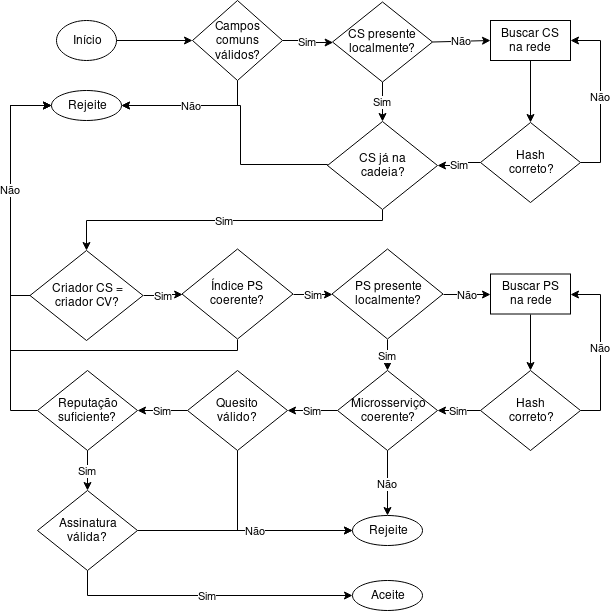
\includegraphics[width=0.8\textwidth]{imagens/validacao_cv.png}
\begin{center}
        Fonte: Autor.
\end{center}
\label{fig:validacao_cv}
\end{figure}

São validados os campos comuns em primeiro lugar e em seguida busca-se a Confirmação de Serviço ao qual a convocação se destina, garantindo que esta já encontra-se na cadeia. É então verificado que o criador da convocação é realmente o cliente relacionado no contrato e outras características de coerência da acusação, que são o índice da \ac{PS} acusada  e do microsserviço negligenciado serem menores ou iguais à quantidade de \acp{PS} contratadas e à quantidade de microsserviços na proposta em questão, respectivamente; o quesito conter um código de aspecto de violação válido; o cliente ter reputação suficiente para o que estipula como aposta mínima e a suposta assinatura do módulo ser de fato verídica. Se todas as informações são coerentes para o contexto da acusação a transação é considerada válida.
%
Transações de \ac{CV} podem ser respondidas única e exclusivamente por votos oriundos de qualquer grupo de usuários.

\subsection{Voto}
\label{sec:proposta:auditoria:voto}

O voto trata-se da fase subsequente do processo de auditoria. Votos podem ser enviados por todos os tipos de usuários desde que o voto seja condizente com a acusação, ou seja, os dados de monitoração se refiram ao provedor acusado e a infraestrutura em questão seja a mesma. Os votos carregam uma parte específica dos dados criptografados que refletem a monitoração feita por aquele usuário, seja ele cliente ou prestador de serviço e usuários pertencentes a grupos diferentes têm igual importância e chance de afetar o resultado final. Os campos utilizados por essa transação são expressos na Tabela \ref{tabela:voto}.

\begin{table}[ht]
\centering
    \begin{tabular}{|m{0.15\textwidth}|m{0.6\textwidth}|m{0.15\textwidth}|}
    \hline
         \textbf{Campo} & \textbf{Descrição} & \textbf{Tamanho}  \\
         \hline
         \ac{CV} \textit{Hash} & Contém o \textit{Hash} criptográfico da convocação de votação ao qual o voto se destina & 32 \textit{bytes} \\
         \hline
         Valor da aposta & Contém o valor que será apostado por aquele usuário & 2 \textit{bytes} \\
         \hline
         Tamanho da assinatura & Contém o tamanho da assinatura do módulo & 1 \textit{byte} \\
         \hline
         Assinatura & Assinatura do \textit{hash} dos dados com a chave privada do módulo & 70, 71 ou 72 \textit{bytes} \\
         \hline
         Tamanho dos dados & Indica o tamanho do conjunto de dados da votação & 4 \textit{bytes} \\
         \hline
         Dados criptografados & Carrega todos os dados criptografados que servem como prova de monitoração e voto & Variável \\
    \hline
    \end{tabular}
    \caption{Campos da transação de Voto}
    \label{tabela:voto}
\end{table}

O primeiro campo indica o \textit{hash} da transação de convocação de votação correspondente ao qual o voto é destinado. O segundo campo indica o valor em pontos de reputação que será apostado pelo usuário no processo de votação ao qual o voto se refere, devendo obrigatoriamente ser maior ou igual ao valor de aposta mínima definido pelo usuário acusador. O terceiro campo indica o tamanho da assinatura seguinte, estando presente por propósitos de serialização. O quarto campo consiste da assinatura criada pelo módulo para esse conjunto de dados específico, atestando que sua origem é legítima. O quinto campo indica o tamanho dos dados e novamente existe por propósitos de serialização. O sexto campo compreende os dados criptografados criados e traduzidos pelo módulo destinados a servir como prova e voto.

%
A validação da transação de voto é relativamente simples, primeiramente os campos comuns são verificados e em seguida carrega-se a convocação de votação relativa para que seja possível atestar se o período de votação ainda continua aberto e se a votação indicada de fato existe. Verifica-se então se o usuário tem reputação suficiente para realizar a aposta indicada no voto e por fim, é verificada se a suposta assinatura do módulo está correta. Se todas os requisitos de validação são atendidos a transação é considerada válida. A transação de voto pode apenas ser referenciada por uma transação de \ac{VT} criada por um usuário ou prestador de serviço.

% entretanto um valor que decide a influência que um voto terá comparado aos outros é a frequência e quantidade de monitorações contidas nos dados anexados.

\subsection{Veredito e Transferências}
\label{sec:proposta:auditoria:vt}

A parte final da fase de auditoria e consequentemente de um ciclo completo do protocolo é a construção do veredito a respeito da violação do contrato, as alterações dos pontos de reputação para os usuários envolvidos, seja em caso de acréscimo ou decréscimo no total individual. Uma vez que o período de votação acabou e existe certa quantidade de votos na cadeia é possível calcular, baseando-se nos dados fornecidos pelos usuários envolvidos, a probabilidade real de um provedor ter violado o contrato. Para tal, os dados probabilísticos de violações de cada usuário são usados para construir uma média de probabilidade, que representa a visão concêntrica e indutiva da rede sobre aquele nível de quebra. Através do uso da média e do desvio padrão dos dados oriundos dos usuários, é possível inferir quais as chances do nível e probabilidade de quebra apontadas pelo acusador realmente acontecerem. A partir dessa inferência cria-se o veredito a respeito da culpa do prestador de serviço em questão. Se o provedor for considerado culpado ele perde o valor mínimo da aposta que é dividido entre o acusador e todos os votantes, caso contrário, quem perde é o cliente acusador. No caso de perda do cliente, sua reputação é dividida apenas entre os votantes e não com o acusado, isto por motivos de segurança tratados na Seção \ref{sec:ameacas_gerais}. 

%
À medida que certos usuários que não forneceram dados tão assertivos ou parecidos com o restante da rede recebem menos pontos de reputação, os usuários que contribuíram positivamente recebem mais. Essa redistribuição é baseada na média, assim a distância da probabilidade individual para a média rege quanto um usuário ganha ou perde.

% TODO: média? Pq?

%
% Devido ao consenso distribuído, a maioria dos usuários deve concordar com o veredito e as redistribuições, consequentemente transações de veredito devem ser escritas e divulgadas na rede. 

%
% A transação de \ac{VT}, como o nome sugere, contém o veredito sobre quem foi declarado desonesto e um conjunto de acréscimos ou decréscimos nos pontos de reputação destinados a cada usuário, indicando quanto será repassado individualmente no final do processo, valor esse que pode ser maior ou menor que o inicial apostado. Essa transação referencia todos os votos e utiliza a soma de seus respectivos valores como definição do montante total a ser dividido. 

%
Esse tipo de transação deve ser criado exclusivamente pelo usuário responsável pela acusação ou pelo prestador de serviço acusado, uma vez que necessariamente um dos dois - que tende a ser o vencedor - terá interesse na conclusão do processo de votação, obtenção do veredito e redivisão dos pontos de reputação. Junto a transação de \ac{VT} deve também ser enviada a chave pública que ambos os usuários obtiveram do módulo e que é capaz de descriptografar os dados, isso para que os outros participantes possam também ver os dados de votação e chegar ao mesmo veredito. Se a chave pública informada não está correta a transação não passa no processo de validação. Se ambos os participantes permitidos enviarem uma transação de \ac{VT} é validada a que estiver correta e se ambas estiverem corretas, será adicionada na bloco a primeira recebida. 
%
%
%
Para evitar que o cliente acusador ou o prestador acusado deliberadamente criem um atraso indefinido para o envio do veredito contendo a chave pública, é estipulado um limite de tempo para que esse tipo de transação seja enviada, sendo esse proporcional ao \textit{locktime} da votação em questão. Caso nenhum veredito seja recebido durante o período estipulado a votação é considerada inválida.

%
Os outros participantes devem também calcular o veredito e redivisões apenas para realizar o processo de validação dessas transações. Para tal, ao receber a transação repassada de algum outro nó, um usuário qualquer que deseja confirmar o veredito deve procurar todos os votos referenciados por essa transação na cadeia e utilizar a chave pública informada para descriptografar os dados de cada um. Possuindo os dados claros, basta executar o cálculo de veredito e redivisão e comparar o resultado obtido com os dados presentes na transação enviada e se estiverem de acordo a transação é considerada verídica e honesta e pode ser repassada. A transação de \ac{VT} é o fim do processo de auditoria de uma infraestrutura e portanto não há nenhuma outra transação existente que pode referenciá-la.

\begin{table}[ht]
\centering
    \begin{tabular}{|m{0.15\textwidth}|m{0.6\textwidth}|m{0.15\textwidth}|}
    \hline
         \textbf{Campo} & \textbf{Descrição} & \textbf{Tamanho}  \\
         \hline
         \ac{CV} \textit{Hash} & Contém o \textit{Hash} criptográfico da convocação de votação & 32 \textit{bytes} \\
         \hline
         Chave pública da votação & Indica qual a chave pública da votação atual & 33 \textit{bytes} \\
         \hline
         Quantidade de Votos & Contém a quantidade de votos recebidos na votação & 2 \textit{bytes}\\
         \hline
         \textit{Hashs} dos Votos & Contém os \textit{hashs} de todas as transações de voto enviadas para a votação & Variável\\
         \hline
         Transferências & Vetor contendo a alteração em reputação conferida a cada usuário participante da votação & Variável \\
    \hline
    \end{tabular}
    \caption{Campos da transação de Veredito e transferências}
    \label{tabela:vt}
\end{table}

O primeiro campo contém o \textit{hash} da transação de convocação de votação referente ao veredito e está presente para que seja possível encontrar corretamente a acusação na cadeia. O segundo campo consiste na chave pública de votação capaz de descriptografar os dados de todos os votos enviados. O terceiro campo contém a quantidade de votos recebidos para aquela votação e está presente por motivos de serialização. O quarto campo trata-se de um vetor com os \textit{hashs} de todos os votos recebidos, de modo que qualquer usuário consiga encontrá-los para realizar o cálculo verificatório do veredito. O quinto e último campo compreende o vetor de transferências contendo um valor de adição ou subtração no montante individual de reputação de cada participante para cada voto respectivamente relacionado no campo quatro. Os possíveis valores que a transferência para um usuário pode assumir não possui um máximo, porém o mínimo é definido como o valor de sua aposta negativado, quando o mesmo perde tudo que apostou. A forma de validação dessa transação é mostrada no fluxograma da Figura \ref{fig:validacao_vt}.

\begin{figure}[ht!]
\caption{Fluxograma para validação de Veredito e Transferências.}
\centering
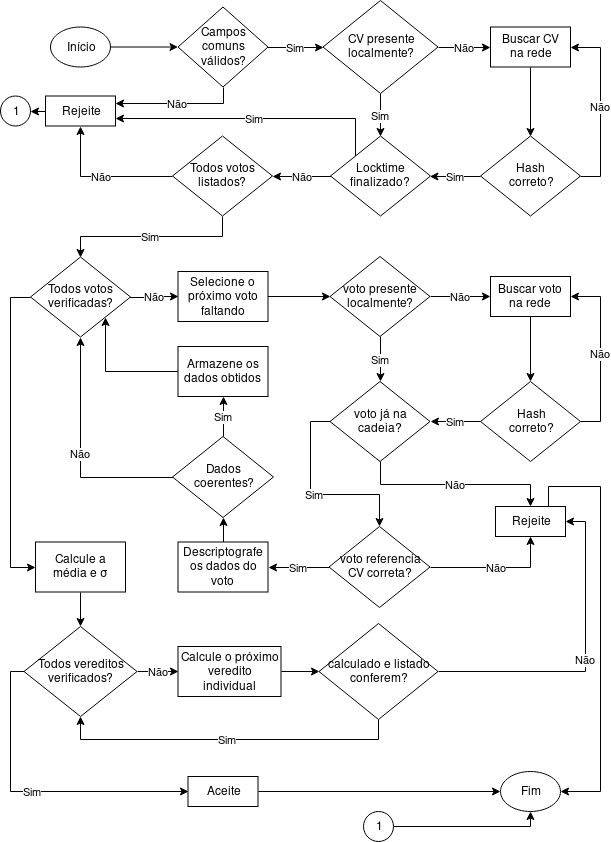
\includegraphics[width=0.8\textwidth]{imagens/validacao_vt.png}
\begin{center}
        Fonte: Autor.
\end{center}
\label{fig:validacao_vt}
\end{figure}

Para a validação da transação de \ac{VT}, da mesma forma que nas outras, primeiramente são verificados os campos comuns e caso esses estejam corretos é carregada a acusação relativa. Com a transação recuperada é verificado se o \textit{locktime} já se encerrou - se novos votos não podem mais ser recebidos - e em caso positivo se verifica se o recebimento de vereditos ainda é permitido para aquela votação. Em caso positivo, é verificado se todos os votos enviados e registrados na cadeia estão sendo referenciados no veredito. Após tais checagens, são então recuperados todos os votos listados, garantindo que todos os votos referenciados estão também presentes na cadeia. Cada voto é então descriptografado utilizando-se da chave pública de descriptografia e se os dados contidos forem válidos para a votação estes são armazenados, caso contrário apenas não são levados em conta no veredito e naturalmente nas transferências. Por fim, ao conhecer os dados de todos os votos que serão usados, gera-se o veredito e as transferências individuais para cada usuário participante. Se todas as verificações resultarem em sucesso e os vereditos individuais calculados na verificação coincidirem com os previamente listados pelo usuário que publicou a transação de \ac{VT} então a transação é considerada válida.
%
Assim, todo o processo de votação pode ser visto como galhos que se expandem a partir de uma confirmação de serviço e que encontram seu fim com a gravação de uma transação de veredito no Blockchain.

\subsection{Cálculo do Veredito}
\label{subsec:calc_veredito}

Para que seja possível distribuir os valores em reputação entre os diferentes usuários é necessária a existência de uma forma de cálculo dos valores apropriados para cada um, esta Seção tem por objetivo propor uma forma de divisão dos valores de reputação com base na assertividade dos dados apresentados pelos usuários.

%
Primeiramente, recebe-se a acusação do usuário, todos os votos respectivos e a chave capaz de descriptografá-los. Após todos os dados verificados, são extraídas as informações de monitoração em si para todo o período. Os dados individuais de cada usuário são então ordenados de maneira crescente com base nos resultados em porcentagem dos testes. Dessa forma, as primeiras posições de cada conjunto serão ocupadas por suas quebras mais severas e quanto mais perto das posições finais do conjunto, menor será a intensidade das mesmas. Se eventualmente houverem monitorações que não apresentam quebras, essas logicamente ocuparão as últimas posições. A ordenação dos dados pode ser realizada dessa maneira pois a análise de intensidade e quantidade de quebras é feita com base na distribuição de das violações no período e não essencialmente em sua ordem cronológica de ocorrência original.

Então é calculada a dissimilaridade dos dados apresentados por diferentes usuários em relação a acusação feita pelo cliente. Para tal, cada voto é comparado individualmente com os dados da acusação, processo que se inicia através da extração da quantidade de quebras detectadas tanto na acusação do cliente quanto no voto a ser comparado, sendo que os registros não considerados quebras são os cuja porcentagem excede um certo limiar alto predefinido, como noventa ou noventa e cinco porcento de recursos disponibilizados, por exemplo. 

%
Após a identificação da quantidade de quebras nos dados ordenados dos conjuntos são utilizadas duas formas distintas de cálculo de dissimilaridade para formar o resultado final. Assim, sendo $q_a$ e $q_vi$ a quantidade de quebras identificadas na acusação e voto respectivamente, as diferentes dissimilaridades são calculadas por:

\begin{equation}
    D_1(A, V_i, q_a, q_{vi}) = \sum_{j = 1}^{q_a} \sum_{k = 1}^{q_{vi}} \sqrt{(A_j - V_ik)^2}
\end{equation}

\begin{equation}
    D_2(A, V_i, q_a, q_{vi}) = \sum_{j = 1}^{q_a} \sum_{k = 1}^{q_a} \sqrt{(A_j - V_ik)^2}
\end{equation}

Na qual, $A$ é o conjunto de dados de monitoração da acusação, $V_i$ é conjunto de dados de um determinado voto, $A_j$ e $V_ik$ são registros pertencentes aos respectivos conjuntos e $D_1$ e $D_2$ são as medidas de dissimilaridade parcial. A dissimilaridade final é dada pela média aritmética das parciais. 

%
O uso de duas formas diferentes para o cálculo da dissimilaridade é empregado justamente pelas diferentes características que são levantadas por cada uma deles. A primeira forma $D_1$ compara individualmente cada quebra da acusação com cada outra quebra presente no voto, apresentando uma visão completa acerca das diferenças de intensidade de violação em ambos os conjuntos. Essa abordagem é interessante porque não se restringe unicamente à quantidade de quebras apontadas pelo cliente acusador quando a existência de mais ou menos violações nos votos podem indicar que o contexto de monitoração do cliente ou do voto não é condizente com o real. Entretanto, essa forma naturalmente supervaloriza o peso da quantidade de quebras no cálculo da dissimilaridade, de forma que um voto pode ter padrões de quebra muito semelhantes aos da acusação e possuir dissimilaridade maior que outros menos parecidos, apenas por uma pequena diferença na quantidade de quebras.

%
Para tratar tais condições é utilizada a segunda forma de dissimilaridade $D_2$ que utiliza única e exclusivamente a quantidade de violações apontadas pela acusação para realizar a comparação. Assim, foca-se principalmente na diferença de intensidade dos dados, assegurando que contextos semelhantes porém com número de quebras diferente não sejam considerados muito dispares. A junção das duas formas de cálculo garante portanto que a dissimilaridade cresce proporcionalmente a medida que a quantidade e intensidade de quebras difere nos dados apresentados, sem necessariamente adotar uma visão binária das informações.

%
Após obtidas as dissimilaridades individuais de todos os votos em relação à acusação, utiliza-se a mediana desses resultados como visão geral da rede sobre o quão distantes os dados se localizam. É usada a mediana ao invés da média de dissimilaridade pois a segunda é muito suscetível a variação decorrente de valores distantes do padrão, o que prejudicaria a precisão do veredito e das distribuições. Por fim, para gerar o veredito apenas é verificado se a mediana é menor que um determinado valor $\alpha$ de dissimilaridade e caso positivo o usuário é considerado vitorioso, caso contrário o prestador é definido como vencedor. O valor de $\alpha$ pode ser definido empiricamente ou com base nos próprios dados, ditando o que seria o limiar de semelhança dos votos com a acusação para que essa seja considerada verídica.

Por fim para o cálculo das distribuições de reputação são utilizadas principalmente as informações referentes ao valor apostado pelo usuário e de quão próximo da mediana de dissimilaridade seus dados ficaram. Após o veredito, o acusado perde toda a sua reputação referente à aposta mínima e esta é dividida entre os votantes. Assim, se inicialmente o total de reputação apostado era formado por $n$ usuários incluindo o perdedor, agora o mesmo total será dividido por $n - 1$ justamente devido à sua derrota. Contudo, o valor individual é ponderado e a lógica por trás da ponderação é que todo usuário perde uma parte do que ele deveria receber como recompensa de acordo com a falta de precisão dos seus dados e recebe uma parcela do que todos os outros usuários perderam. A perda recebida por cada usuário acontece de forma proporcional à porcentagem representada pelo desvio de seus dados em relação ao somatório de desvio de todos os votos. A fração que cada usuário recebe da perda de outros é proporcional a porcentagem que sua aposta representa do total de reputação da votação. Logo, se todos os usuários convergirem precisamente sobre os dados, todos recebem apenas proporcionalmente ao quanto investiram e caso haja divergência nos votos os menos próximos ao consenso recebem menos. 

%
Como o usuário acusador não possui nenhum valor de dissimilaridade relacionado aos seus dados - pois as dissimilaridades são justamente calculadas em relação a sua acusação - este apenas recebe parcelas das perdas dos outros e para contrabalancear o fato de que o mesmo não perde reputação graças a imprecisão, evita-se que ele receba porcentagens maiores e então recebe apenas como base o mesmo valor que apostou. Praticamente então, o valor dividido entre os votantes é dado pelo valor total de reputação, menos a aposta inicial do cliente, dividido agora por $n - 2$ usuários. 

Por fim, sendo $D_f$ a dissimilaridade final entre a acusação e um voto; $\Tilde{d}$ a mediana de todas as dissimilaridades; $D_t$ a soma das distâncias de dissimilaridades individuais até a mediana; $u$ a quantidade de usuários votantes; $v$ a quantidade de votos; $a_i$ a aposta de um usuário $i$ qualquer; $t$ o total de reputação daquela votação, as divisões de reputação são dadas pelas equações: 

\begin{equation}
    D_f(A, V_i) = \frac{D_1(A, V_i, q_a, q_{vi}) + D_2(A, V_i, q_a, q_{vi})}{2}
\end{equation}

\begin{equation}
    D_t = \sum_{i = 1}^v D_f(A, V_i) - \Tilde{d}
\end{equation}

\begin{equation}
    R_a = a_a + \sum_{i = 0, a \neq i}^u \frac{a_i}{t}(1 - \frac{D_f(A, V_i)}{D_t}) 
\end{equation}

\begin{equation}
    R_i = a_i - \frac{a_i}{t}(1 - \frac{D_f(A, V_i)}{D_t}) + \sum_{j = 0, j \neq i}^u \frac{a_j}{t}(1 - \frac{D_f(A, V_j)}{D_t}) 
\end{equation}

Nas quais $R_i$ é a reputação de um usuário qualquer e $R_a$ trata-se da reputação do usuário acusador, caso o mesmo vença a votação. Nota-se ainda que o resultado é dado na forma de um novo valor de reputação, entretanto a transação de \ac{VT} espera um valor de adição ou subtração no total individual. Para calcular tal variação basta executar a subtração $R_i - a_i$ e então inseri-la na posição correta do vetor na transação.

Essa forma de cálculo do veredito e das distribuições apresenta de maneira justa uma ponderação de assertividade dos dados e valor apostado na conferência de créditos ou débitos aos usuários. Entretanto, como já mencionado nessa seção, trata-se de uma forma inicial e básica de distribuição que pode eventualmente em trabalhos futuros ser refinada ou modificada, de modo a melhor se adequar a situações do mundo real. De maneira generalizada, o protocolo trata também de maneira agnóstica o cálculo dos vereditos, facilitando o emprego de novas abordagens interessantes desde que sejam previamente testadas e aprovadas em uma análise de ameaças teórica.

% A medida de dissimilaridade é interessante para o presente caso pois garante singularidade e precisão para a diferenciação dos dados apresentados, compreendendo características como quantidade de quebras e intensidade das mesmas em uma medida única e eficiente.

%
            

% \section{Transações especiais}
% \label{sec:proposta:especiais}

% O protocolo depende necessariamente de outros formatos de transação que não estão relacionados nem com o estabelecimento de contratos e nem com a auditoria dos mesmos, os objetivos dessas transações são estabelecer configurações e divulgações públicas de informações, nesta seção são abordados essas transações e suas características. Transações especiais, da mesma forma que as regulares, utilizam o conjunto de campos comuns apontados na Seção \ref{tabela:dados_comuns}.

\section{Publicação de Certificado}
\label{sec:proposta:certificado}

O protocolo utiliza uma transação especial que trata-se da \ac{PC} e como o nome sugere, é utilizada para divulgar aos outros participantes da rede a existência de um certificado pertencente ao usuário criador da transação. Certificados, como apontado na Seção \ref{sec:proposta:definicoes}, devem ser conferidos por alguma forma de entidade central a todos os usuários que desejam ingressar na rede como prestadores de serviço e após recebê-lo, esse novo usuário deve obrigatoriamente publicá-lo para que o restante da rede possa averiguar sua participação no grupo de prestadores de serviço. Os campos individuais dessa transação são expressos na tabela \ref{tabela:pc}.

\begin{table}[ht]
\centering
    \begin{tabular}{|m{0.15\textwidth}|m{0.6\textwidth}|m{0.15\textwidth}|}
    \hline
         \textbf{Campo} & \textbf{Descrição} & \textbf{Tamanho}  \\
         \hline
         Tamanho Assinatura & Contém o tamanho da assinatura seguinte & 1 \textit{byte} \\
         \hline
         Assinatura & Contém a assinatura da entidade certificadora & 70, 71 ou 72 \textit{bytes} \\
    \hline
    \end{tabular}
    \caption{Campos da transação de Publicação de certificado}
    \label{tabela:pc}
\end{table}

A única informação que deve efetivamente ser carregada por essa transação é o certificado em si, que trata-se fundamentalmente de uma assinatura de um determinado órgão considerado confiável. Assim, o primeiro campo indica o tamanho da assinatura e o segundo campo a assinatura em si. O prestador de serviço deve então referenciar essa transação toda vez que criar uma \ac{PS} para que seja possível garantir a integridade e validade do envio de uma proposta. Nenhuma transação de nenhum outro usuário pode referenciar uma transação de publicação de certificado. 

% \subsection{Atualização de Certificado}
% \label{sec:proposta:atualizacao_cert}

% A segunda transação adicional importante para o protocolo é a \ac{AC} de um determinado prestador de serviço. É importante considerar que embora a transação chame-se atualização de certificado não é o certificado em si que é atualizado, mas sim a chave que anteriormente era certificada por ele. Em aplicações reais que funcionam sobre protocolos como HTTP não trata-se de uma prática comum a autoatualização de certificados, na qual o recebedor do mesmo consegue modificar sua chave pública sem violar a validade do certificado em si, porém no contexto da proposta tal ação é possível. Para tal, objetivando atualizar sua chave pública por qualquer motivo, relacionado ou não com segurança, o prestador de serviço apenas precisa provar que possui a chave privada que foi inicialmente certificada.

\section{Exemplo de Utilização do Alvorada}
\label{sec:proposta:exemplo}

Para a apresentação do exemplo prático - com informações reais no decorrer dessa seção - uma adaptação da Figura \ref{fig:cenario_execucao} foi feita para a construção da Figura \ref{fig:exemplo_execucao}, entretanto todas as formas de representação e legendas foram mantidas. Nesse novo esquema todas as fases do protocolo são mostradas utilizando dados de um contexto real de execução, porém em menor escala.

\begin{figure}[ht!]
\caption{Exemplo prático de execução.}
\centering
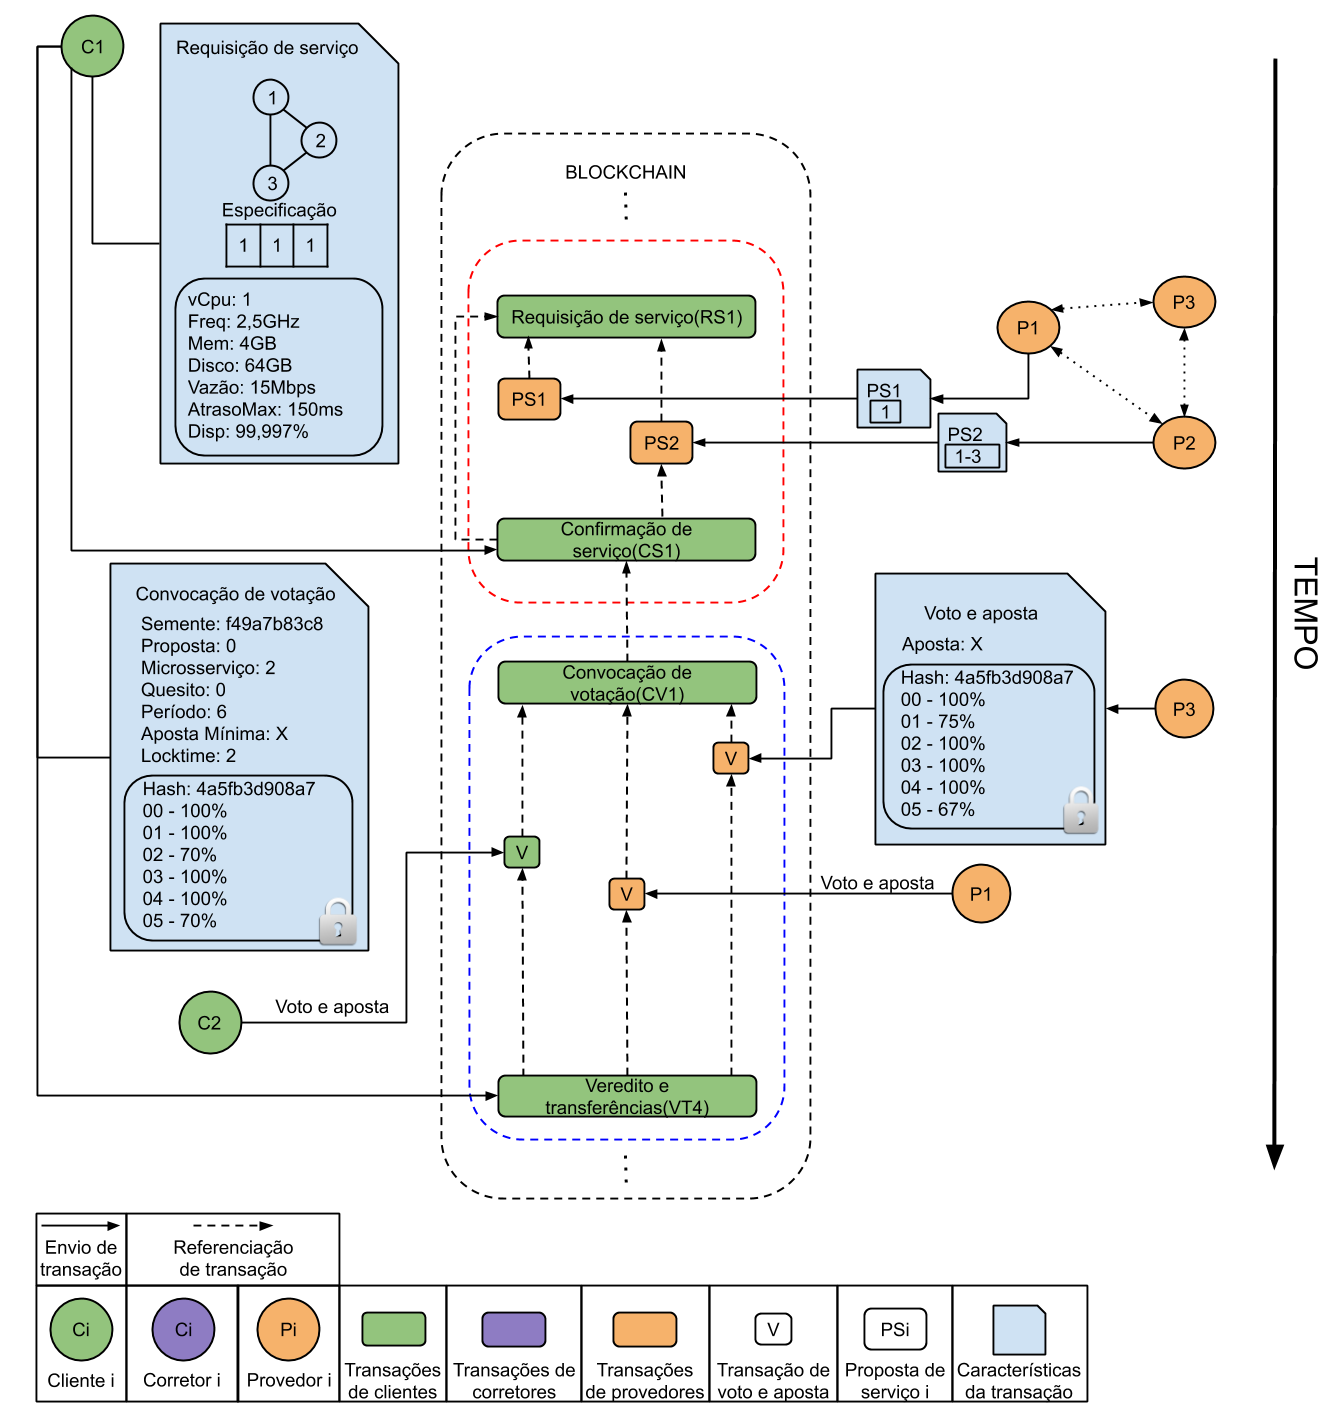
\includegraphics[width=1\textwidth]{imagens/exemplo_execucao.png}
\begin{center}
        Fonte: Autor.
\end{center}
\label{fig:exemplo_execucao}
\end{figure}

Um cliente $C1$ deseja fazer uma transação para alocar um conjunto de microsserviços de sua aplicação. Para tal, a transação $RS1$ é criada especificando como se dá a organização de seus microsserviços - através de um grafo - e qual é a infraestrutura escolhida para cada um deles. Nesse caso as características físicas escolhidas foram: uma \textit{vCpu}, com frequência de 2,5GHz, memória principal de 4GB, disco de 64GB, vazão de 15Mbps, atraso máximo de comunicação 150ms e disponibilidade de 99,997\%. $C1$ deseja que todos os seus microsserviços usem a mesma infraestrutura então a referenciação para tal é feita no vetor de relação dos microsserviços. $C1$ então envia sua transação para a rede e uma vez que foi inserida na cadeia, prestadores de serviço podem enviar suas propostas. Os provedores $P1$ e $P2$ decidem enviar propostas de serviço que atendam ao requisitado pelo cliente. O primeiro se propõe a suprir apenas o microsserviço um, enquanto o segundo propõe suprir a totalidade do serviço, sendo os microsserviços um, dois e três. Os preços de cada uma das propostas foram omitidos porque não interferem no funcionamento do protocolo e sim apenas na escolha do cliente. $C1$ então se interessa pela proposta $PS2$ do provedor $P2$ e como ela contempla todos os seus microsserviços não há necessidade de criação de uma prolongação de requisição. Uma transação de confirmação de serviço é criada pelo cliente referenciando a $PS2$ que foi escolhida. Assim, a elaboração do contrato que atende às necessidades do cliente foi concluída, envolvendo todos os dados referentes à \acp{SLI} e \acp{SLO}, bem como o preço pago por $C1$.

%
Durante a execução dos processos iniciais do estabelecimento do contrato descritos até o momento, os provedores $P1$, $P2$ e um terceiro provedor $P3$ já executam a inter-monitoração através do método de disfarce citado na Seção \ref{sec:cenario_execucao}.

%
Eventualmente, $C1$ recebe um alerta de seu módulo de monitoração informando que uma quebra no contrato foi detectada na realização de um teste infringindo a quantidade de poder de computação disponível em certa porcentagem. Como $C1$ não recebeu o que estava estabelecido no contrato, o provedor deve ser responsabilizado e punido. Primeiramente, $C1$ realiza todo o processo explanado na Seção \ref{fig:votacao_detalhada} para obter os dados que serviram como sustento de sua acusação. Então, objetivando averiguar e punir o provedor em questão, deve ser criada uma transação de convocação de votação. Nessa transação, $C1$ especifica que o contrato violado trata-se de $CS1$, sua semente criptografada é $f49a7b83c8$,  o serviço que foi violado é o prestado pela $PS2$, a infraestrutura em questão é a do segundo microsserviço na requisição e que o período de monitoração utilizado é de seis testes. O valor mínimo da aposta que deve ser pago para participar da votação também é adicionado nas informações dessa transação. O \textit{locktime}, que indica por quanto tempo a transação pode ser referenciada é definido como dois, dessa forma participantes podem enviar seus votos até que dois blocos sejam adicionados após o bloco da transação atual. Votos que forem enviados após os dois blocos de altura aceitos do \textit{locktime} serão rejeitados.

%
A partir do momento de publicação da convocação de votação de $C1$ na cadeia, participantes que possuem dados criptográficos de monitoração a respeito do provedor que está sendo acusado e da infraestrutura relacionada podem enviar seus votos sobre a veracidade ou não da acusação. No exemplo, $P1$, $P3$ e um cliente $C2$ - que possui um contrato ativo com $P2$ - decidem enviar votos para a convocação de $C1$. No voto de $P3$, que é tomado como exemplo, foram encontrados níveis de violação semelhantes aos do usuário em duas das últimas seis monitorações e o valor apostado foi o mínimo.

%
Assim que o período de votação se fecha o usuário acusador ou o provedor acusado podem enviar uma transação de veredito e transferência de modo a finalizar o processo. No exemplo é suposto que da mesma forma que $P3$, tanto $C2$ quanto $P1$ apostaram apenas o mínimo e possuem dados parecidos, que atestam a veracidade da acusação do usuário e portanto consideram $P2$ como culpado. No presente exemplo o usuário acusador é o único a enviar a transação de \ac{VT} e nela é informado que o provedor foi julgado responsável e que todos os outros quatro usuários corretos ($C1$, $C2$, $P1$ e $P3$) recebem além do valor inicial apostado, o valor da aposta mínima referente a $P2$ dividido entre todos. Assim, se encerra a fase de auditoria do contrato, na qual o culpado é punido e os participantes corretos recompensados por meio de reputação aos olhos da rede.

% \section{Ameaças ao Protocolo}
% \label{sec:proposta:ameacas}

% Primeiramente, por tratar-se de uma rede de Blockchain, acomete-se sobre o protocolo todas as dificuldades e ameaças recorrentes das mesmas. O conjunto de ameaças pode ser identificado como segue:
% \begin{itemize}

    % \item O primeiro ponto de impacto direto sobre sistema é claramente a escolha do método de consenso, que por si só possui cenários em que o funcionamento é ameaçado e esses, de forma semelhante, decorrem sobre a presente proposta como um todo.

%     \item Como a carteira digital desempenha um grande papel em manter os usuários realizando suas obrigações e na manutenção das votações, outra grande ameaça é a sua violação, que pode ser quebrada ou modificada de modo a realizar transações e outras ações de forma anômala ou prejudicial para a rede. Esse tipo de ação pode ser realizada visando ganhos individuais e ameaça a reputação de todos os outros participantes, sendo portanto um fator de preocupação importante.

% %
%     \item Semelhante à carteira, o protocolo depende de um oráculo, que trata-se do sistema de monitoração distribuído e sendo de desenvolvimento próprio ou de terceiros pode ser usado por participantes maliciosos, no caso da existência de falhas ou aberturas, para moldar a monitoração aos seus interesses.

% %
%     \item Ainda no tocante à monitoração, se de alguma forma for possível que o provedor monitorado descubra as aplicações disfarçadas, este pode alocar ambientes estáveis que não refletem o dos usuários reais, descaracterizando todo o propósito e eficácia da monitoração em si. Mesmo que um certo grupo de usuários maliciosos exista na rede, esta ainda consegue operar. 

% %
%     \item No contexto específico da votação, o limiar para possibilidade de resultados corretos é de no máximo 51\% de nós fraudulentos. Entretanto, como exemplificado ao longo desse capítulo, uma série de medidas são tomadas para que não seja possível adulterar ou prejudicar o funcionamento do sistema.

% \end{itemize}

\section{Trabalhos Relacionados}
\label{sec:trabalhos_relacionados}

Esta seção tem por objetivo relacionar trabalhos que tratam do problema da elaboração e auditoria de \acp{SLA}, tanto no contexto de \ac{IaaS} quanto de outras áreas proeminentes da computação, com enfoque no uso de Blockchain.
%
Não foram encontrados trabalhos que tratam da alocação de infraestruturas especificamente para microsserviços por meio de Blockchain, porém no recente trabalho de \citeonline{blockchain_iaas} foi proposta uma rede de Blockchain baseada no \textit{Ethereum} para a alocação e monitoração de \ac{IaaS} em termos gerais, cujo propósito é criar um mercado público para infraestruturas. Primeiramente, utiliza-se uma rede secundária encarregada da implantação e operação dos serviços, negociações e dados de monitoração, enquanto a Blockchain armazena contratos inteligentes e resultados de decisões de violação. Os contratos inteligentes são utilizados como representação de possíveis serviços, que são negociáveis para atender às necessidades do cliente. A decisão sobre violações é feita por uma entidade centralizada através dos dados de monitoração e apenas se comentam possibilidades de um modelo distribuído para a realização desse processo.

%
O trabalho de \citeonline{blockchain_scas} busca novamente utilizar o \textit{Ethereum} e os contratos inteligentes para automatizar o processo de elaboração de contratos \ac{SCaaS}, onde pequenas empresas e locações domésticas poderiam alugar parte de suas infraestruturas de rede para provedores de internet móvel. A concessão do equipamento acontece por meio de modelos de contratos inteligentes que, são acordados por ambas as partes e baseiam-se em pagamentos periódicos. Todo o processo de monitoração é regido apenas pelo provedor, que pode aplicar multas e eventualmente cancelar o contrato devido a quebra.

\citeonline{blockchain_5gslicer} propôs uma rede de Blockchain que em conjunto com outras tecnologias atua como um \textit{slicer} para internet móvel 5G, destinando-se ao de fornecimento de infraestruturas através de contratos inteligentes para empresas de diversos ramos, em específico para dispositivos de automação em indústrias. A alocação pode ser feita por demanda através do Blockchain sendo necessária a existência de um oráculo que forneça dados de monitoração, voltados para cobrança ou compensação monetária em casos de violação de uma das partes.

O trabalho de \cite{blockchain:blockchain_as} propõe um sistema baseado em Blockchain para conferir pontuações distintas para provedores de internet, o sistema também faz uso de um oráculo que garante informações a respeito da rede e do serviço fornecido. É utilizada uma forma de conferência baseada em dois atores, no qual as informações de ambos devem ser assertivas e iguais a respeito dos dados reunidos pelo oráculo. Um terceiro ator verificador também pode ser invocado em casos de tentativas de fraude por uma das partes. Formas de penalização e tratamento de diferentes possíveis ataques e ameaças à rede também são tratadas.

A proposta de \citeonline{blockchain_cdn} trata-se de uma rede de Blockchain baseada no \textit{Hyperledger Fabric}, voltada para o estabelecimento de contratos colaborativos para a provisão de conteúdo em \acp{CDN}. São utilizadas múltiplas cadeias destinadas a negociação, distribuição ao longo da rede e monitoração, sendo que para a última sugere-se apenas um breve modelo de funcionamento. Clientes, provedores de conteúdo e facilitadores técnicos são os atores, sendo que clientes escrevem buscas, que transformadas em contratos definem o conteúdo buscado e preferências. Provedores criam novos contratos, que referenciam os anteriores oferecendo um serviço, para que facilitadores técnicos, de forma semelhante, criem contratos derivados que definem características técnicas da entrega e preços.

%
O presente trabalho difere dos anteriores por propor um protocolo capaz de não apenas auxiliar a elaboração de contratos de \ac{IaaS} voltados para microsserviços, mas também sistematicamente ranquear os provedores de acordo com sua credibilidade. Esta é publicamente visível graças ao sistema de pontos de reputação, característica até então não observada em outras propostas e que exerce ajuda significativa no processo de escolha. Além disso, é proposto um sistema de auditoria dos \acp{SLA} que baseia-se no monitoramento descentralizado e atestável, convergindo para um mapeamento dinâmico da qualidade de serviço dos provedores. 

\section{Considerações Parciais}
\label{sec:proposta:consideracoes}

Este capítulo dedica-se então a definição de um conjunto de formalismos teóricos que regem o funcionamento do protocolo, indicando como o mesmo utiliza as tecnologias subjacentes para estabelecer uma plataforma funcional voltada ao estabelecimento de contratos e a possibilidade de suas auditorias.

%
A definição do protocolo relaciona como de fato são organizadas as transações, suas estruturas e hierarquia de aparecimento na cadeia. Os aspectos principais instituídos para o módulo e para a carteira servem para auxiliar no mantimento do formato dos dados e interações com a rede, embora as próprias diretivas de validação garantam a coerência. A definição de características básicas da rede juntamente aos algoritmos de verificação para cada transação criam um perfil de comportamento que deve ser adotado pelos usuários para que estejam em comunhão com o coletivo, evitando rejeição de suas ações.

%
% No Capitulo \ref{ch:ameaças}, são então discutidas possíveis ameaças ao protocolo de acordo com as políticas de funcionamento 


% TODO: indique as considerações do capítulo.